\documentclass[oneside,a4paper,english,links]{amca}

\usepackage[utf8]{inputenc}% para ver los acentos OK
\usepackage{verbatim}
\usepackage{graphicx}
\usepackage{amsmath,amsfonts}
\usepackage[table]{xcolor}
\usepackage{graphicx}
\usepackage{wrapfig} %for graphics in parallel text
\usepackage{color} %for highlighting
\newcommand{\hilight}[1]{\colorbox{yellow}{#1}}%for highlighting
\usepackage{gensymb} %for degree symbol
\usepackage[colorinlistoftodos,textsize=tiny]{todonotes}
%-------
% para resaltar
\usepackage{color} 
\usepackage{soul}  
%-------
\usepackage{subcaption}  % parasubfigure
\usepackage{float}
%------- multicolumnas
\usepackage{multicol}
\usepackage[table]{xcolor}
%\usepackage[spanish,activeacute]{babel} show error, is for utilizing Spanish packets

\title{The tennis racket theorem, an analysis of the intermediate axis theorem - cambio github - cambio en overleaf}


\author{Nicolas Trivisonno$^1$, Luciano Garelli$^1$, Mario Storti}

%\author[1]{Nicolas Trivisonno, Luciano Garelli, Mario Storti}


\affil{CIMEC Centro de Investigación de Métodos Computacionales, UNL, CONICET, FICH, Col. Ruta 168 s/n, Predio Conicet "Dr Alberto Cassano", 3000 Santa Fe, Argentina, http://www.cimec.org.ar}

%\affil[1]{CIMEC Centro de Investigación de Métodos Computacionales, UNL, CONICET, FICH, Col. Ruta 168 s/n, Predio Conicet "Dr Alberto Cassano", 3000 Santa Fe, Argentina, http://www.cimec.org.ar}


%\affil[2]{Escuela de Ingeniería Mecánica, FCEIA - UNR. Beruti 2109, Rosario, Argentina}


\begin{document}
\vspace{2.5cm} %3cm
\maketitle


\begin{keywords}
Tennis racket theorem, Intermediate axis theorem, Dzhanibekov effect, Principal axis inestability, Wingnut effect
\end{keywords}

%%%%%%%%%%%%%%%%%%%%%%%%%%%%%%%%%%%%%%%%
\begin{abstract} % este fue el que presentamos, pero lo modificamos
The aim of this paper is to reproduce the phenomenon of the intermediate axes theorem also known as the Dzhanibekov effect or the Tennis Racket effect. A Rigid Body Dynamic (RBD) model with six degree of freedom (6DOF) was developed to reproduce the Euler Equations of motion. Two configuration of object were analyzed in order to reproduce the intermediate axis effect. Also a mathematical approach was performed in order to present the physics of the precession.
\end{abstract}

\begin{comment}
\begin{abstract} % este fue el que presentamos, pero lo modificamos
The aim of this paper is to reproduce the phenomenon of the intermediate axes theorem also known as the Dzhanibekov effect or the Tennis Racket effect. A Rigid Body Dynamic (RBD) model with six degree of freedom (6DOF) was developed using quaternions for the mathematical modeling.
Several simulations were perform in order to analyze the effect in  different directions and in various scenarios such us environments with and without gravity.
\end{abstract}
\end{comment}

\begin{comment}
otro tipo de abstract
\begin{abstract}
The intermediate axis theorem also known as tennis racket theorem or Dzhanibekov effect says that in a asymmetrical top object (three different principal inertia moments, where $I_1<I_2<I_3$) the spin around the first and third principal is stable, but if the object rounds around the second inertia un peculiar efecto surge en la trayectoria descripta por el mismo. is unstable. The aim of this paper is to reproduce this effect in any direction and in different atmospheres. (con y sin gravedad). Several simulations were perform in a Rigid Body Dynamics model with six degrees of freedom (RBD-6DOF) utilizing quaternions for the mathematical representation.
\end{abstract}
\end{comment}

%-------------------------------------------

\begin{comment}
El viscosímetro de Couette es un dispositivo que se utiliza para cuantificar la viscosidad de un dado fluido. Consta de dos cilindros concéntricos rotantes donde se relaciona la viscosidad con el torque requerido para girar los mismos a una velocidad conocida. A bajas velocidades de rotación el flujo se comporta laminar y estacionario. Sin embargo, cuando se incrementa la velocidad de rotación del cilindro interior por sobre un dado límite, los flujos de Couette comienzan a ser inestables y emergen vórtices toroidales axisimétricos, conocidos como flujo de vórtices de Taylor. Este patrón estable de flujo secundario se caracteriza mediante el número adimensional conocido como Número de Taylor.
El objetivo del presente trabajo es visualizar el fenómeno de inestabilidad de Taylor-Couette para distintos Números de Taylor mediante la utilización de técnicas de CFD (por sus siglas en inglés) [1][2]. Como primera instancia se estudia la relación entre los parámetros involucrados para obtener la solución exacta de la velocidad como así también el perfil de la misma, comparándose con la solución numérica [3]. Luego, se realizan varias simulaciones numéricas a diferentes Números de Taylor’s con la intención de registrar el patrón de flujo secundario generado. Para hacer frente a las cuestiones numéricas se utilizó la plataforma Salome para el pre y pos-proceso y la plataforma OpenFoam [4] para cuestiones de CFD.
\end{comment}

%\end{document}

\section{Introducción}

El teorema del eje intermedio tambi\'en conocido como teorema de la raqueta de tenis enuncia que sobre un objeto denominado \textit{asymmetrical top} (tres momentos principales de inercia diferentes, donde $I_1<I_2<I_3$), su rotaci\'on respecto a la primer y tercer direcci\'on principal es estable, mientras que el giro respecto al segundo eje de inercia, produce un efecto extra\~no y per\'iodico debido a la inestabilidad de dicha revoluci\'on.

%Actually, the intermediate axis theorem also known as tennis racket theorem effect says that in a asymmetrical top object (three different principal inertia moments,  where $I_1<I_2<I_3$) the spin around the first and third principal inertia is stable, but if the object rounds around the second inertia this motion will realice a weird an periodic movement due to an inestability in its spin.

El enunciado del teorema del eje intermedio se viene estudiando desde larga data por ser un problema de la mec\'anica cl\'asica, \cite{poinsot1851theorie}, \cite{landau1976mechanics}, \cite{ashbaugh1991twisting}, y hasta alcanz\'o la categor\'ia de secreto de estado para algunas potencias mundiales durante la carrera espacial. El mismo adquiri\'o tal relevancia cuando se realiz\'o la misi\'on Soyuz T-13\footnote{Misi\'on realizada en 1985 donde fue una de las proezas de las misiones aeroespaciales debido al acoplamiento manual y la posterior recuperaci\'on de la estaci\'on espacial Salyut-7 la cual se encontraba orbitando a la deriva.} ya que mientras se realizaba la reparaci\'on para volver a poner operativa la estaci\'on espacial, el comandante Dzhanibekov presenci\'o la misteriosa trayectoria sobre un tuerca mariposa mientras realizaba el mantenimiento del equipo, por lo que tambi\'en se suele denominar efecto Dzhanibekov o efecto Wingnut por la denominaci\'on de dicha tuerca en ingl\'es.

Si bien el teorema del eje intermedio se conoce desde hace tiempo ya que corresponde al an\'alisis tradicional de la mec\'anica cl\'asica, debido a su efecto tan peculiar y poco intuitivo, el mismo no deja de asombrar a cualquiera que presencia ese misterioso comportamiento. El objetivo del trabajo es reproducir dicho efecto mediante un modelo de RBD con 6DOF el cual utiliza cuaterniones para la representaci\'on matem\'atica. Como beneficio indirecto, realizando dicho ejemplo se valida la implementaci\'on del modelo y se evidencia la potencialidad de la representaci\'on matem\'atica por medio de cuaterniones ya que permiten reproducir lanzamientos en direcci\'on vertical, situaci\'on que no puede realizarse si se utilizan \'angulos de Euler debido a la singularidad conocida como \textit{gimbal-lack}.

El presente trabajo est\'a compuesto por una primer secci\'on en la cual se presentan una clasificaci\'on de os objetos en funci\'on de sus momentos de inercia, Sec.(\ref{sec:Descripci\'on}). Luego, se procede a analizar las ecuaciones de Euler para las distintas clasificaciones de objetos, donde se analiza la f\'isica del movimiento de precesi\'on: Sec.(\ref{sec:cinemat_An\'alsis_momentos_angulares_Aplicaciones_Ec_Euler_symmetrical_top}) y Sec.(\ref{sec:cinemat_asymmetrical_top_precesion}). Y por \'ultimo, se reproduce y analiza la inestabilidad del eje intermedio, Sec.(\ref{sec:resultados}).

%-------------------------------------------
\section{Descripci\'on}
\label{sec:Descripci\'on}

\textbf{Tensor de inercia:} La inercia de un cuerpo se encuentra definida por 6 valores los cuales conforman un tensor sim\'etrico de orden tensorial 2, es decir sea el tensor de inercia I, entonces $I\;\in\;CT(2)$\footnote{CT hace referencia a Cartensian Tensor}, Ec.(\ref{eq:cinematica_tensor_inercia}). Como todo CT(2), dicho tensor puede transformarse a un tensor diagonal si las direcciones de los ejes son correctamente elegidas, dicho proceso se conoce como diagonalizaci\'on y los elementos de la diagonal son a los momentos principales de inercia, los cuales corresponden a las inercias en las direcciones seleccionadas para diagonalizar el tensor\footnote{Este proceso es el que se realiza cuando se obtienen los autovalores y autovectores de un CT(2)}.

\begin{equation}
    I_{ij} = I_{ji}=
    \begin{bmatrix}
    I_{xx} & I_{xy} & I_{xz}\\ 
    I_{xy} & I_{yy} & I_{yk}\\
    I_{xz} & I_{yz} & I_{kk}\\
    \end{bmatrix}
    \label{eq:cinematica_tensor_inercia}
\end{equation}

En otras palabras al realizar la diagonalizaci\'on de $I\in CT(2)$ se obtendr\'an dos tensores: $I_d, v$, Ec.(\ref{eq:cinematica_tensores_obteniados_al_diagonalizar_tensor_inercial}) siendo $I_d,v\in CT(2)$. $I_d$ es un tensor diagonal, cuyos elementos diagonales son los momentos principales de inercia, y los vectores columnas del tensor $v$ son las direcciones principales de inercia.

\begin{equation}
    I_d =
    \begin{bmatrix}
    I_1 & 0 & 0\\ 
    0 & I_{2} & 0\\
    0 & 0 & I_{3}\\
    \end{bmatrix}
    v =
    \begin{bmatrix}
   v_{11} & v_{21} & v_{31}\\ 
    v_{12} & v_{22} & v_{32}\\ 
    \underbrace{v_{13}}_{v_1} & \underbrace{v_{23}}_{v_2} & \underbrace{v_{33}}_{v_3}\\ 
    \end{bmatrix}
    \label{eq:cinematica_tensores_obteniados_al_diagonalizar_tensor_inercial}
\end{equation}

\noindent Adem\'as por convenci\'on se los organiza de modo que $I_1>I_2>I_3$ donde estas inercias tienen la particularidad que ninguna  puede superar a la suma de las otras dos, por ejem:

\begin{equation}
    I_1+I_2 \geq I_3
\end{equation}

Los momentos de inercia caracterizan la rotaci\'on de un cuerpo en una dada direcci\'on. Dependiendo de como sean dichos momentos de inercia se pueden clasificar a los cuerpos en distintos grupos, a saber:

\begin{itemize}
    \item inercias todas id\'enticas: $I_1=I_2= I_3$, se denomina objeto \textit{spherical top}
    \item dos inercias iguales y la tercera no: $I_1=I_2 \neq I_3$, se denomina objeto \textit{symmetrical top}
    \item todas inercias distintas entre s\'i: $I_1\neq I_2\neq I_3$, se denomina objeto \textit{asymmetrical top}
\end{itemize}

Siempre que un cuerpo gire sobre uno de sus ejes principales, entonces el vector momento se encontrar\'a alineado con el vector velocidad. Cuando el vector velocidad (el cual est\'a dado por el elipsoide de la energ\'ia cin\'enita, \textit{KE}) deja de ser colineal con el vector momento entonces se produce el movimiento de \texttt{precesi\'on}. Por lo tanto se puede definir a la \textit{precesi\'on} como el par\'ametro que indica cuan desalineado se encuentra vector velocidad con respecto al eje principal. En la Sec.(\ref{sec:cinemat_An\'alsis_momentos_angulares_Aplicaciones_Ec_Euler_symmetrical_top}) se ampl\'ia el concepto de \texttt{precesi\'on}.


%-------------------------------------------
\section{Modelo - An\'alsis de momentos angulares - Aplicaciones de las Ecuaciones de Euler}
\label{sec:cinemat_modelo_An\'alsis_momentos_angulares_Aplicaciones_Ec_Euler}

El momento angular est\'a dado por la ecuaci\'on $\Vec{M}=\underline{\underline{I}} \Vec{\Omega}$, donde el vector momento es proporcional a la velocidad angular  siempre y cuando el cuerpo se encuentre rotando sobre los ejes principales de inercia, es decir en dicho caso la velocidad angular se encuentra alineada con el vector momento. Por otro lado, si el cuerpo gira en cualquier otra direcci\'on entonces la velocidad angular no se encontrar\'a alineada con el vector momento y se producir\'a un movimiento conocido como \texttt{precesi\'on}.

En las siguentes secciones se procede a analizar distintas soluciones para un sistema en el cual no act\'uan esfuerzos externos, tanto Fuerzas como Momentos. La trayectoria descripta por el cuerpo estar\'a dada por la evoluci\'on temporal de las ecuaciones de movimiento, Ec.(\ref{eq:cinemat_ODEs_vel_angular_sin_torques_externos}), las cuales se resumen en las 6ODE's (Ordinary Differential Equation, 'Ecuaciones Diferenciales Ordinarias'), \cite{landau1976mechanics}. Como el foco del estudio es la rotaci\'on, se elude el an\'alisis para la traslaci\'on, estudi\'andose solamente la rotaci\'on. Adem\'as se omiten las contribuciones debido a los torques externos.


\begin{equation}
\begin{cases}
    \dot{\Omega}_1= \frac{1}{I_{1}}\Sigma \Vec{\tau}^{ext}_1+\frac{\left(I_2-I_3\right)}{I_1}\Omega_3\Omega_2\\
    \dot{\Omega}_2=\frac{1}{I_{2}}\Sigma \Vec{\tau}^{ext}_2+\frac{\left(I_3-I_1\right)}{I_2}\Omega_1\Omega_3\\
    \dot{\Omega}_3=\frac{1}{I_{3}}\Sigma \Vec{\tau}^{ext}_3+\frac{\left(I_1-I_2\right)}{I_3}\Omega_2\Omega_1\\
\end{cases}
\begin{cases}
    \dot{\Omega}_1=\frac{\left(I_2-I_3\right)}{I_1}\Omega_3\Omega_2\\
    \dot{\Omega}_2=\frac{\left(I_3-I_1\right)}{I_2}\Omega_1\Omega_3\\
    \dot{\Omega}_3=\frac{\left(I_1-I_2\right)}{I_3}\Omega_2\Omega_1\\
    \end{cases}
    \label{eq:cinemat_ODEs_vel_angular_sin_torques_externos}
\end{equation}

\subsection{Spherical Top}
\label{sec:cinemat_An\'alsis_momentos_angulares_Aplicaciones_Ec_Euler_spherical_top}

En la presente situaci\'on el objeto tiene las inercias id\'enticas, $I_1=I_2=I_3$, por lo cual, las soluciones de la ODE ser\'an constantes que depender\'an de las condiciones iniciales del objeto,  Ec.(\ref{eq:cinemat_ODEs_vel_angular_sin_torques_externos_spherical_top}). 

\begin{equation}
\begin{cases}
    \dot{\Omega}_1=\frac{\left(I_1-I_1\right)}{I_1}\Omega_3\Omega_2\\
    \dot{\Omega}_2=\frac{\left(I_1-I_1\right)}{I_2}\Omega_1\Omega_3\\
    \dot{\Omega}_3=\frac{\left(I_1-I_1\right)}{I_3}\Omega_2\Omega_1\\
    \end{cases}
    \begin{cases}
    \dot{\Omega}_1=0\\
    \dot{\Omega}_2=0\\
    \dot{\Omega}_3=0\\
    \end{cases}
        \begin{cases}
    {\Omega}_1=C_1\\
    {\Omega}_2=C_2\\
    {\Omega}_3=C_3\\
    \end{cases}
    \label{eq:cinemat_ODEs_vel_angular_sin_torques_externos_spherical_top}
\end{equation}


\subsection{Symmetrical top}
\label{sec:cinemat_An\'alsis_momentos_angulares_Aplicaciones_Ec_Euler_symmetrical_top}

Los cuerpos symmetrical top son los cuerpos que poseen dos momentos de inercia similares y un $3^{er}$ momento de inercia diferente, es decir $I_1=I_2\neq I_3$. De la Ec.(\ref{eq:cinemat_ODEs_vel_angular_sin_torques_externos}), aplicamos la igualdad en la simetr\'ia y se arriba a la Ec.(\ref{eq:cinemat_ODEs_vel_angular_sin_torques_ecternos_symmetrical_top}).


\begin{equation}
\begin{cases}
    \dot{\Omega}_1=\frac{\left(I_1-I_3\right)}{I_1}\Omega_3\Omega_2\\
    \dot{\Omega}_2=\frac{\left(I_3-I_1\right)}{I_1}\Omega_1\Omega_3\\
    \dot{\Omega}_3=\frac{\left(I_1-I_2\right)}{I_3}\Omega_2\Omega_1\\
    \end{cases}
    \begin{cases}
    \dot{\Omega}_1=\frac{\left(I_1-I_3\right)}{I_1}\Omega_3\Omega_2\\
    \dot{\Omega}_2=\frac{\left(I_3-I_1\right)}{I_1}\Omega_1\Omega_3\\
    \dot{\Omega}_3=\frac{\left(0\right)}{I_3}\Omega_2\Omega_1\\
    \end{cases}
        \begin{cases}
    \dot{\Omega}_1=\frac{\left(I_1-I_3\right)}{I_1}\Omega_3\Omega_2\\
    \dot{\Omega}_2=\frac{\left(I_3-I_1\right)}{I_1}\Omega_1\Omega_3\\
    \dot{\Omega}_3=0\\
    \end{cases}
    \label{eq:cinemat_ODEs_vel_angular_sin_torques_ecternos_symmetrical_top}
\end{equation}

Donde $\Omega_3$ resulta ser un valor constante $\Omega_3=C_1$ y por lo tanto el producto de una constante por $\Omega_3$ tambi\'en ser\'a una constante, la cual se denomina $w$. El t\'ermino de la ecuaci\'on de $\Omega_1$ ser\'a $-w$ por tener ser $(I_1-I_3)=-(I_3-I_1)$.

\begin{equation}
            \begin{cases}
    \dot{\Omega}_1=\frac{\left(I_1-I_3\right)}{I_1}\Omega_3\Omega_2\\
    \dot{\Omega}_2=\underbrace{\frac{\left(I_3-I_1\right)}{I_1}\Omega_3}_{c_2\cdot\Omega_3=w}\Omega_1\\
    \Omega_3=C_1\\
    \end{cases}
    \label{eq:cinemat_ODEs_vel_angular_sin_torques_ecternos_symmetrical_top_omega3_c1}
\end{equation}

Por consiguiente el sistema de ecuaciones se resume a un sistema de ecuaciones de dos ecuaciones diferenciales con dos inc\'ognitas.

\begin{equation}
  \begin{cases}
    \dot{\Omega}_1=-w\Omega_2\\
    \dot{\Omega}_2=w\Omega_1\\
    \end{cases}
      \begin{cases}
    \dot{\Omega}_1=\underbrace{0}_a\Omega_1+\underbrace{-w}_b\Omega_2\\
    \dot{\Omega}_2=\underbrace{w}_c\Omega_1+\underbrace{0}_d\Omega_2\\
    \end{cases}
    \label{eq:cinemat_sist_ODE's_acopladas}
\end{equation}

La Ec.(\ref{eq:cinemat_sist_ODE's_acopladas}) es un sistema de ecuaciones diferenciales ordinarias con la particularidad de que sus inc\'ognitas est\'an acopladas y no es posible resolver $\dot{\Omega}_1$ sin resolver $\dot{\Omega}_2$ y viceversa, por lo que se deben resolver las dos simult\'aneamente. Esta situaci\'on ocurre cuando las constantes gen\'ericas b y c son distintas de cero, $b\neq0\wedge c\neq0$. 

Para resolver este tipo de sistemas se puede realizar de forma matricial o sino como en el presente trabajo se opta por resolverlo mediante el m\'etodo que transforma a la primer ecuaci\'on en una ecuaci\'on diferencial de 2do orden, es decir se toma a la primer ecuaci\'on y se deriva respecto a la variable independiente, quedando ahora una ecuaci\'on de segundo orden que involucra  a la primer derivada de la segunda ecuaci\'on, y de esa forma se puede sustituir esta dentro de la anterior.

\begin{equation}
  \begin{cases}
    \dot{\Omega}_1=-w\Omega_2\\
    \dot{\Omega}_2=w\Omega_1\\
    \end{cases}
  \begin{cases}
    \ddot{\Omega}_1=-w\dot{\Omega}_2\\
    \dot{\Omega}_2=w\Omega_1\\
    \end{cases}
  \begin{cases}
    \ddot{\Omega}_1=-w\overbrace{w\Omega_1}^{\dot{\Omega}_2}\\
    \dot{\Omega}_2=w\Omega_1\\
    \end{cases}
      \begin{cases}
    \ddot{\Omega}_1=-w^2\Omega_1
    \end{cases}
      \begin{cases}
    \ddot{\Omega}_1+w^2\Omega_1=0
    \end{cases}
    \label{eq:cinemat_sistema_eq_dif_copladas}
\end{equation}

De esta forma se logra transformar la Ec.(\ref{eq:cinemat_sistema_eq_dif_copladas}) en una ecuaci\'on ordinaria de segundo orden homogenea y a coeficientes constantes. La soluci\'on general de la misma est\'a compuesta por dos soluciones linealmente independientes (LI) de la forma $y_H=C_1\;y_1(t)+C_2\;y_2(t)$. El m\'etodo para calcular dichas soluciones es proponer la soluci\'on Ec.(\ref{eq:cinemat_sol_propuesta_ODE_2do_homegenea_coef_cts}) ya que sus derivadas ser\'an siendo la misma funci\'on.

\begin{equation}
    \begin{split}
        y(t)&=e^{(rt)}\\
        \dot{y}(t)&= r\;e^{(rt)}\\
        \ddot{y}(t)&= r^2\;e^{(rt)}
    \end{split}
    \label{eq:cinemat_sol_propuesta_ODE_2do_homegenea_coef_cts}
\end{equation}

 Al reemplazar la Ec.(\ref{eq:cinemat_sol_propuesta_ODE_2do_homegenea_coef_cts}) que contiene la soluci\'on propuesta y sus derivadas en la Ec.(\ref{eq:cinemat_raices_sol_ODE2dorden}) se arriba a:

\begin{equation}
    \begin{split}
        r^2\;e^{(rt)}+w^2e^{(rt)}=0\\
        \left(r^2+w^2\right)e^{(rt)}=0
    \end{split}
    \label{eq:cinemat_raices_sol_ODE2dorden}
\end{equation}

Como la funci\'on exponencial es asint\'otica en 0, la funci\'on $e^{(rx)}$ nunca alcanzar\'a dicho valor, por lo que la \'unica forma que la Ec.(\ref{eq:cinemat_raices_sol_ODE2dorden}) sea nula es que el polinomio de $2^{do}$ grado sea nulo. Para esto se procede a calcular las raices.

\begin{equation}
    \frac{-b\pm \sqrt{b^2-4\cdot a \cdot c}}{2\cdot a}=    \frac{-0\pm \sqrt{0-4\cdot w^2}}{2}=\frac{\pm \sqrt{(-1)\cdot4\cdot w^2}}{2}=\frac{\pm \sqrt{i^2\cdot4\cdot w^2}}{2}=\frac{\pm 2wi}{2}=\pm wi
    \label{eq:cinemat_raiz_resolvente}
\end{equation}

Por lo que la soluci\'on general de la Ec.(\ref{eq:cinemat_sist_ODE's_acopladas}) ser\'a:

\begin{equation}
  \Omega_{1_{(t)}}=C_1 e^{r_1t}+C_2 e^{r_2t}=C_1 e^{2wit}+C_2 e^{-2wit}  
    \label{eq:cinemat_eq_general_omega1}
\end{equation}
  
Expresando la exponencial imaginaria mediante las funciones trigonom\'etricas $\sin()$ y $\cos()$, la Ec.(\ref{eq:cinemat_eq_general_omega1}) queda:

\begin{equation}
  \Omega_{1_{(t)}} = C_1 cos(wt) + C_2 sin(wt)
  \label{eq:cinemat_sol_omega_1}
\end{equation}

Una vez obtenida la Ec.(\ref{eq:cinemat_sol_omega_1}) se puede reemplazar en la Ec.(\ref{eq:cinemat_sist_ODE's_acopladas}) para calcular la velocidad angular restante, se detalla adem\'as la sustituci\'on para resolver la integral.

\begin{equation}
\begin{split}
    \dot{\Omega}_{2_{(t)}}=w \Omega_1 = w \left[\overbrace{C_1 cos(wt) + C_2 sin(wt)}^{\Omega_{1_{t}}}\right]\\
    \Omega_{2_{(t)}}=\int \dot{\Omega}_{2_{(t)}} dt = \int w\; C_1\; cos(wt) dt +\int w\;C_2\; sin(wt) dt\\
    \Omega_{2_{(t)}}=\int C_1 cos(u) du + \int C_2 sin(u) du \qquad\qquad u=wt\xrightarrow{}du=w\;dt\\
    \Omega_{2_{(t)}}=C_1 sin(u) - C_2 cos(u)\\
    \Omega_{2_{(t)}}=C_1 sin(wt) - C_2 cos(wt)
\end{split}
\label{eq:cinemat_sol_omega_2}
\end{equation}

Finalmente con la Ec.(\ref{eq:cinemat_sol_omega_1}) y Ec.(\ref{eq:cinemat_sol_omega_2}) se obtienen las soluciones del sistema acoplado, Ec.(\ref{eq:cinemat_sist_ODE's_acopladas}), siendo este:

\begin{equation}
    \begin{cases}
     \Omega_{1_{(t)}} = C_1 cos(wt) + C_2 sin(wt)\\
    \Omega_{2_{(t)}}=C_1 sin(wt) - C_2cos(wt)
    \end{cases}
    \label{eq:cinemat_sol_precesion_nico}
\end{equation}

Para el c\'alculo de las constantes inicializamos el sistema de modo que $\Omega_{1_{(0)}}=A$ y $\Omega_{2_{(0)}}=0$.

\begin{equation}
    \begin{cases}
    \Omega_{1_{(0)}} = C_1 \overbrace{cos(w\;0)}^{=1} + C_2 \overbrace{sin(w\;0)}^{=0}\\
    \Omega_{2_{(0)}}=C_1 \overbrace{sin(w\;0)}^{=0} - C_2\overbrace{cos(w\;0)}^{=1}   
    \end{cases}
    \begin{cases}
    A = C_1 \\
    0= - C_2   
    \end{cases}
    \label{eq:cinemat_inicializacion_ODEs_precesion}
\end{equation}

\begin{equation}
    \boxed{
    \begin{split}
    \Omega_{1_{(t)}} = A \;cos(w\;t)\\
    \Omega_{2_{(t)}} = A \;sin(w\;t)
    \end{split}}
    \label{eq:cinemat_resu_omega1_omega2}
\end{equation}

La Ec.(\ref{eq:cinemat_resu_omega1_omega2}) modela un movimiento arm\'onico en dos dimensiones el cual describe la trayectoria curva, donde $A$ es la amplitud, y $\omega$ la frecuencia. En rigor de verdad la frecuencia es $f=\frac{w}{2\pi}$ y $\omega$ es la velocidad angular de rotaci\'on. Es decir el movimiento descripto es per\'iodico, ya que al cabo de un tiempo el vector vuelve a su posici\'on inicial y comienza nuevamente el ciclo. En otras palabras $\omega$ es la velocidad con la que va cambiando el vector velocidad angular $\vec{\Omega}$ y por ende el eje instant\'aneo de rotaci\'on. A dicho fen\'omeno se lo conoce como fen\'omeno de \texttt{precesi\'on} y se define como el movimiento asociado al cambio de direcci\'on en el espacio que experimenta el eje instantaneo de rotaci\'on de un cuerpo, donde la velocidad de dicho cambio es la velocidad de precesi\'on $\Omega_{pr}$. La Ec.(\ref{eq:cinemat_velocidad_precesion}) detalla esta cuesti\'on.

\begin{equation}
    \Omega_{pr}= \tilde{C}\;\Omega_3 = \overbrace{\left(\frac{I_3-I_1}{I_1} \right)}^{\tilde{C}}\Omega_3=\omega 
    \label{eq:cinemat_velocidad_precesion}
\end{equation}

De esta forma se reformula la Ec.(\ref{eq:cinemat_velocidad_precesion}) present\'andose con la velocidad de precesi\'on $\Omega_{pr}$.

\begin{equation}
    \boxed{
    \begin{split}
    \Omega_{1_{(t)}} = A \;cos\left(\Omega_{pr}\;t\right)\\
    \Omega_{2_{(t)}} = A \;sin\left(\Omega_{pr}\;t\right)
    \end{split}}\label{eq:cinemat_resu_omega1_omega2_con_vel_precesion}
\end{equation}

Continuando Ec.(\ref{eq:cinemat_resu_omega1_omega2_con_vel_precesion}) y Ec.(\ref{eq:cinemat_ODEs_vel_angular_sin_torques_ecternos_symmetrical_top_omega3_c1}) se concluye que la velocidad de rotaci\'on del cuerpo es:

\begin{equation}
    \vec{\Omega}=
\begin{bmatrix}
\Omega_1\\
\Omega_2\\
\Omega_3
\end{bmatrix}=
\begin{bmatrix}
A \;cos\left(\Omega_{pr}\;t\right)\\
A \;sin\left(\Omega_{pr}\;t\right)\\
C_1
\end{bmatrix}    
\label{eq:cinemat_resu_omega_vectorial_precesion}
\end{equation}

As\'i pues, la Ec.(\ref{eq:cinemat_resu_omega_vectorial_precesion}) presenta en forma general la velocidad angular del objeto. Se aprecia que $\vec{\Omega}=\vec{\Omega}_{(t)}$ var\'ia instante a instante, es decir, es constante respecto a eje principal $x_3$ pero al estar describiendo una circunferencia, el vector $\vec{\Omega}$ estar\'a recorriendo a dicha curva y tomando valores distintos instante a instante; donde la velocidad con la que el vector va recorriendo esa circunferencia se conoce como velocidad de precesi\'on, $\Omega_{pr}$. Se procede a analizar algunas situaciones particulares:

%\newpage

\begin{itemize}
    \item \underline{t=0}\\
\begin{equation}
    \vec{\Omega}=
\begin{bmatrix}
A \;cos\left(\Omega_{pr}\;t\right)\\
A \;sin\left(\Omega_{pr}\;t\right)\\
C_1
\end{bmatrix}=
\begin{bmatrix}
A \;cos\left(\Omega_{pr}\;0\right)\\
A \;sin\left(\Omega_{pr}\;0\right)\\
C_1
\end{bmatrix}=
\begin{bmatrix}
A \\
0 \\
C_1
\end{bmatrix}
\label{eq:omega_t0}
\end{equation}
\end{itemize}


\begin{itemize}
    \item \underline{$t=\frac{\pi}{2\Omega_{pr}}$}\\
\begin{equation}
    \vec{\Omega}=
\begin{bmatrix}
A \;cos\left(\Omega_{pr}\;t\right)\\
A \;sin\left(\Omega_{pr}\;t\right)\\
C_1
\end{bmatrix}=
\begin{bmatrix}
A \;cos\left(\Omega_{pr}\;\frac{\pi}{2\Omega_{pr}}\right)\\
A \;sin\left(\Omega_{pr}\;\frac{\pi}{2\Omega_{pr}}\right)\\
C_1
\end{bmatrix}=
\begin{bmatrix}
0 \\
A \\
C_1
\end{bmatrix}
\label{eq:omega_tpi/2omega}
\end{equation}
\end{itemize}


\begin{figure}[h]
\begin{subfigure}{.55\textwidth}
  \centering
  % include first image
  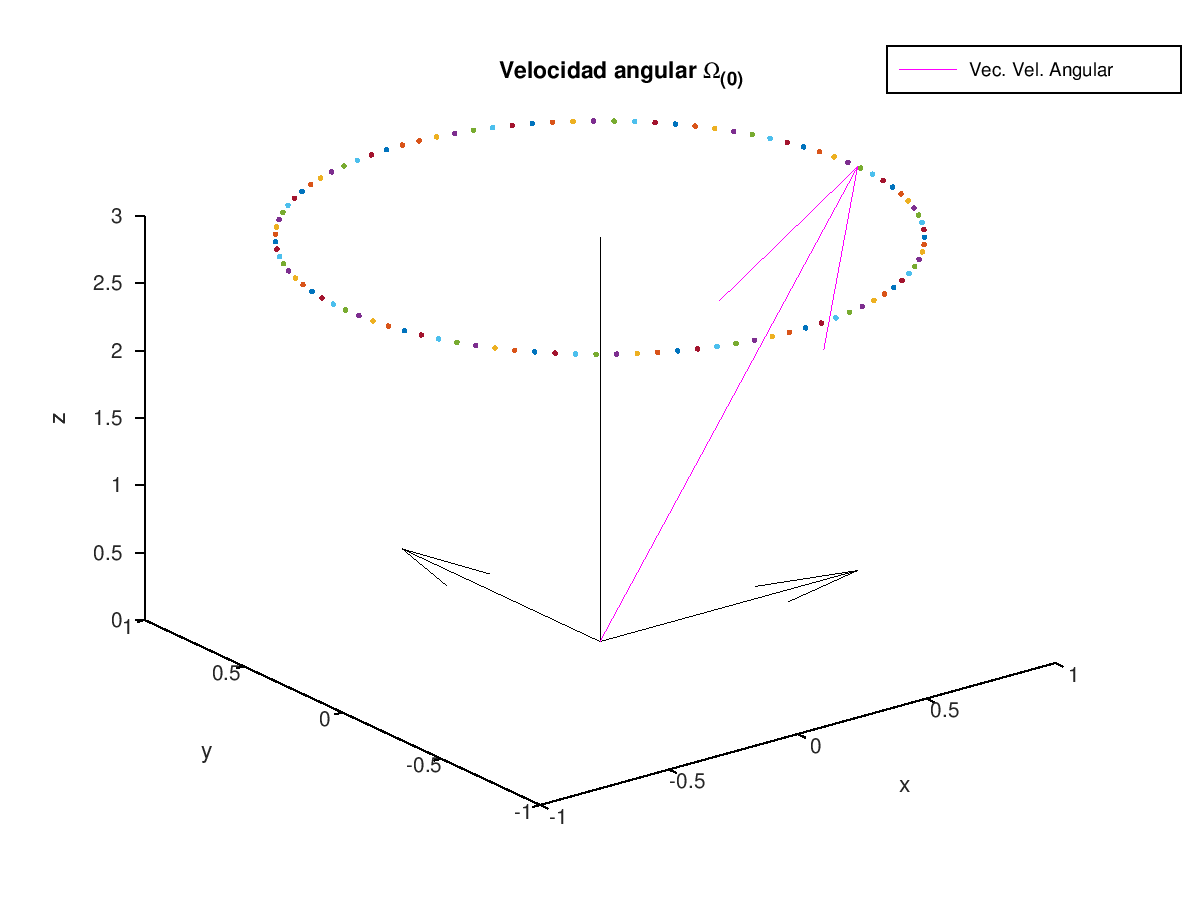
\includegraphics[width=.77\linewidth]{Figuras/omega_t0.png}
  \caption{$\Omega$ en  t = 0}
\label{fig:cinemat_omega_vectorial_t=0}
\end{subfigure}
\begin{subfigure}{.55\textwidth}
  \centering
  % include second image
  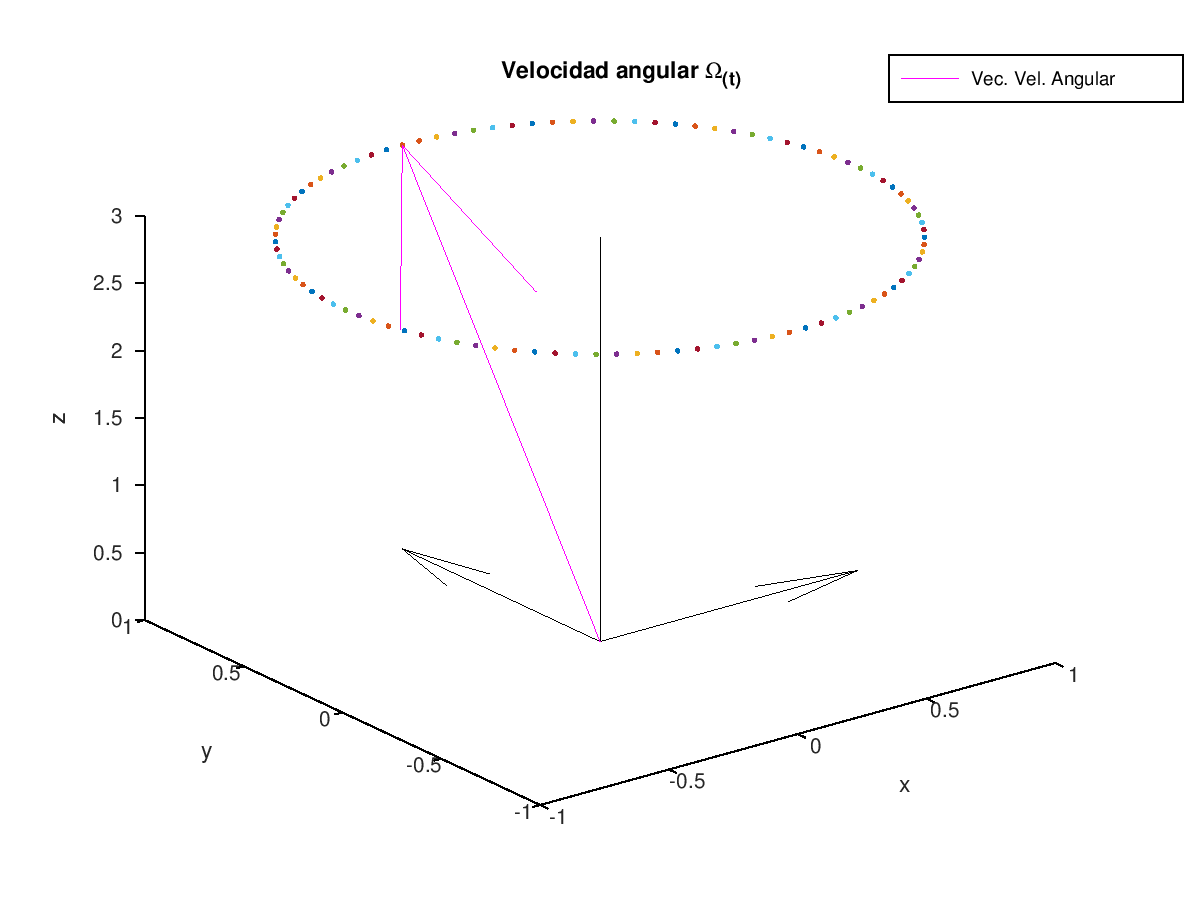
\includegraphics[width=.77\linewidth]{Figuras/omega_t_pi_2omega_prec.png}
  \caption{$\Omega$ en t $=\frac{\pi}{2\Omega_{pr}}$}
\label{fig:cinemat_omega_vectorial_t=pi/(2omega_pr)}
\end{subfigure}
\caption{Vector velocidad angular, $\vec{\Omega}$}
%\label{fig:recorrido_vector_momento_subfigures_matlab_y_video_mario}
\end{figure}

De las Fig.(\ref{fig:cinemat_omega_vectorial_t=0}) y Fig.(\ref{fig:cinemat_omega_vectorial_t=pi/(2omega_pr)}) se aprecia que el vector velocidad angular $\vec{\Omega}$ var\'ia en funci\'on del tiempo, ya que $\Omega_1=\Omega_{(t)}$, idem para $\Omega_2$. No obstante su m\'odulo es constante, Ec.(\ref{eq:cinemat_justif_modulo_omega_cte}). Se demuestra que siendo $A,C_1 \epsilon\; CT(0)$ y por ende la suma de constantes tiene como resultado otra constante, $\tilde{C}\epsilon\; CT(0)$.



\begin{equation}
    \begin{split}
    |\vec{\Omega}|^2&=\Omega_i\;\Omega_j\;\delta_{ij}\\
   |\vec{\Omega}|^2&=\left[A \;cos\left(\Omega_{pr}\;t\right) \right]^2+\left[A \;sin\left(\Omega_{pr}\;t\right) \right]^2+\left[C_1 \right]^2\\
    |\vec{\Omega}|^2&=A^2 \;cos^2\left(\Omega_{pr}\;t\right)+A^2 \;sin^2\left(\Omega_{pr}\;t\right)+C_1^2\\
     |\vec{\Omega}|^2&=A^2 \;\underbrace{\left[ cos^2\left(\Omega_{pr}\;t\right)+ \;sin^2\left(\Omega_{pr}\;t\right)\right]}_{=1}+C_1^2\\
      |\vec{\Omega}|^2&=\underbrace{A^2+C_1^2}_{\tilde{C}}\\
      |\vec{\Omega}|^2&=\tilde{C}
    \end{split}
    \label{eq:cinemat_justif_modulo_omega_cte}
\end{equation}

Se realiza el mismo procedimiento para estudiar el momento, donde se demuestra que si bien el vector momento $\vec{M}$ var\'ia instante a instante, ya que depende de la velocidad angular y anteriormente se demostr\'o dicha dependencia temporal, no obstante su m\'odulo es constante. Se procede a realizar dos ejemplos en los mismos instantes de tiempo anteriores, $t=0$ y $t=\frac{\pi}{2\;\Omega_{pr}}$ 

\begin{equation}
    \vec{M} = M_1 \hat{i} +M_2 \hat{j}+ M_3 \hat{k} 
\end{equation}



\begin{itemize}
    \item \underline{$t=0$:} Recordamos que: 
\begin{equation*}
    \vec{\Omega}_{(0)}=
    \begin{bmatrix}
    A\\
    0\\
    C_1
    \end{bmatrix}
\end{equation*}

\noindent Por lo tanto cuando la matriz de inercia se encuentra diagonalizada el vector momento expresado en la notaci\'on de Einstein ser\'a $\vec{M}_j=I{ij}\Omega_i$

\begin{equation}
    \vec{M}=
\begin{bmatrix}
I_{xx} \Omega_{1(t)} \\
I_{yy} \Omega_{2(t)}  \\
I_{zz}  \Omega_3
\end{bmatrix}\xrightarrow[]{}\vec{M}_{(0)}
\begin{bmatrix}
I_{xx} A \\
    0\\
I_{zz}    C_1
\end{bmatrix}
\label{eq:cinemat_momento_vectorial_t=0}
\end{equation}

\end{itemize}





\begin{itemize}
    \item \underline{$t=\frac{\pi}{2\Omega_{pr}}$:} Recordamos que:
\begin{equation*}
    \vec{\Omega}_{\left(\frac{\pi}{2\Omega_{pr}}\right)}=
    \begin{bmatrix}
    0\\
    A\\
    C_1
    \end{bmatrix}
\end{equation*}

\noindent Por lo tanto cuando la matriz de inercia se encuentra diagonalizada el vector momento expresado en la notaci\'on de Einstein ser\'a $\vec{M}_j=I{ij}\Omega_i$

\begin{equation}
    \vec{M}=
\begin{bmatrix}
I_{xx} \Omega_{1(t)} \\
I_{yy} \Omega_{2(t)}  \\
I_{zz}  \Omega_3
\end{bmatrix}\xrightarrow[]{}\vec{M}_{\left(\frac{\pi}{2\;\Omega_{pr}}\right)}=
\begin{bmatrix}
0\\
I_{yy} A \\
I_{zz}    C_1
\end{bmatrix}
\label{eq:cinemat_momento_vectorial_t=pi/2omegapr}
\end{equation}

\end{itemize}

\begin{figure}[h]
\begin{subfigure}{.55\textwidth}
  \centering
  % include first image
  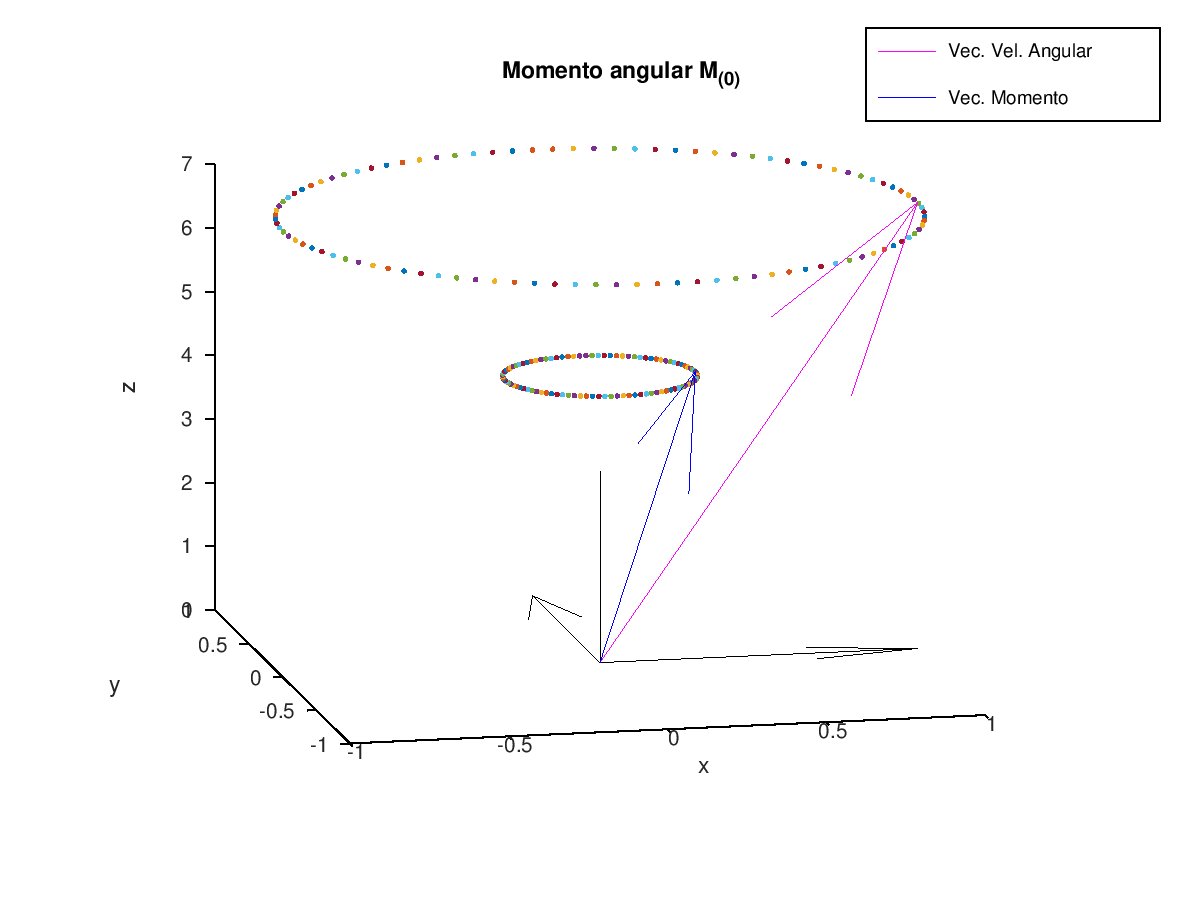
\includegraphics[width=.77\linewidth]{Figuras/momento_t_0.png}
  \caption{$\vec{M}$ en  t = 0}
\label{fig:cinemat_momento_vectorial_t=0}
\end{subfigure}
\begin{subfigure}{.55\textwidth}
  \centering
  % include second image
  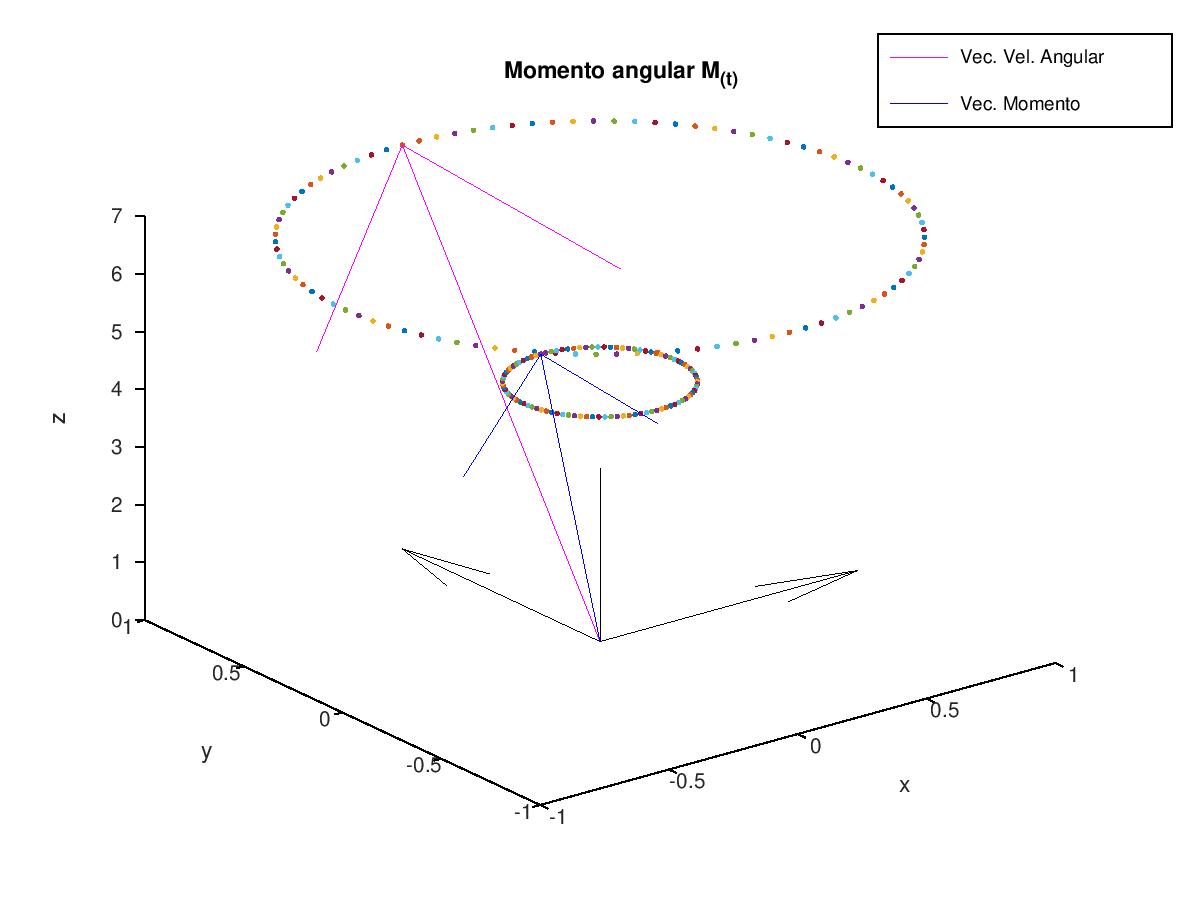
\includegraphics[width=.77\linewidth]{Figuras/momento_t_pi_2omega_prec.png}
  \caption{$\vec{M}$ en t $=\frac{\pi}{2\Omega_{pr}}$}
\label{fig:cinemat_momento_vectorial_t=pi/2omegapr}
\end{subfigure}
\caption{Vector momento angular, $\vec{M}$}
%\label{fig:recorrido_vector_momento_subfigures_matlab_y_video_mario}
\end{figure}

Tanto la Ec.(\ref{eq:cinemat_momento_vectorial_t=0}) y Ec.(\ref{eq:cinemat_momento_vectorial_t=pi/2omegapr}) como tambi\'en la Fig.(\ref{fig:cinemat_momento_vectorial_t=0}) y Fig.(\ref{fig:cinemat_momento_vectorial_t=pi/2omegapr}) manifiestan que el plano de acci\'on de la velocidad angular $\vec{\Omega}$ y el momento $\vec{M}$ es el mismo, y este var\'ia instante a instante. Como se expresa con anterioridad el vector $\vec{\Omega}$ por acci\'on de la precesi\'on va variando instante a instante pero no su m\'odulo y lo mismo ocurre con el vector momento $\vec{M}$, que debido a la diferencia en sus componentes producto de las inercias, no es igual a $\vec{\Omega}$ sino que va acompa\~nando al vector velocidad angular $\vec{\Omega}$. Por \'ultimo se analiza el m\'odulo del vector momento sobre el cual se demuestra que si bien el vector momento var\'ia por tener la dependencia temporal $\vec{M}=\vec{M}_{(t)}$, no obstante su m\'odulo es constante, ya que $A,C_1\;\epsilon CT(0)$ y estos se multiplican por los momentos de inercia que son constante, se arriba a que $|\vec{M}|^2\;\epsilon CT(0)$.

\begin{equation}
\begin{split}
    |\vec{M}|^2&=M^2_1+M^2_2+M^2_3\\
    |\vec{M}|^2&=\left(I_1 \Omega_1 \right)^2+\left(I_2 \Omega_2 \right)^2+\left(I_3 \Omega_3 \right)^2\\
    |\vec{M}|^2&=I_1^2 \Omega_1^2+I_2^2 \Omega_2^2+I_3^2 \Omega_3^2\\
    |\vec{M}|^2&=I_1^2 \left[A \;cos\left(\Omega_{pr}\;t\right) \right]^2+I_2^2 \left[A \;sin\left(\Omega_{pr}\;t\right) \right]^2+I_3^2 \left[C_1 \right]^2\\
    |\vec{M}|^2&=I_1^2 A^2 \;cos^2\left(\Omega_{pr}\;t\right)+I_2^2 A^2 \;sin^2\left(\Omega_{pr}\;t\right)+I_3 C_1 ^2\\
    |\vec{M}|^2&=I_1^2 A^2 \;cos^2\left(\Omega_{pr}\;t\right)+I_2^2 A^2 \;sin^2\left(\Omega_{pr}\;t\right)+I_3^2 C_1 ^2\\
    |\vec{M}|^2&=I_1^2 A^2 \underbrace{\left[ \;cos^2\left(\Omega_{pr}\;t\right)+ \;sin^2\left(\Omega_{pr}\;t\right)\right]}_{=1}+I_3^2 C_1 ^2\\
    |\vec{M}|^2&=\underbrace{I_1^2 A^2 +I_3^2 C_1 ^2}_{\tilde{C}}\\
    |\vec{M}|^2&=\tilde{C}
    \end{split}
    \label{eq:cinemat_justif_modulo_momento_cte}
\end{equation}





\subsection{Asymmetrical Top}
\label{sec:cinemat_asymmetrical_top_precesion}

Ahora se realiza el estudio para un cuerpo donde los tres momentos de inercia son diferentes entre s\'i, es decir $I_1\neq I_2\neq I_3$ y adem\'as $I_1>I_2>I_3$. Si se piensa en funci\'on de la conservaci\'on del momento angular, donde $\vec{M}=\underline{\underline{I}}\;
\vec{\Omega}$ entonces si $|\vec{M}|=C$ al aumentar I$\uparrow$, disminuye $\Omega\;\downarrow$, esto es: I3 ser\'a el menor eje de inercia y por lo tanto tendr\'a la mayor velocidad de rotaci\'on.

\begin{equation}
   \begin{split}    I_1&>I_2>I_3\\
   \Omega_1&<\Omega_2<\Omega_3\\
   \Omega_3&<\Omega_2<\Omega_1\\
   \end{split}
    \label{eq:cinemat_relacion_inercias_vel_angulares}
\end{equation}


La Ec.(\ref{eq:cinemat_energia_momentos_elipsoides_ambos}a) es la ecuaci\'on de la energ\'ia cin\'etica de rotaci\'on, la cual representa todas las configuraciones de modo que el objeto tenga la m\'axima energ\'ia de rotaci\'on para determinadas velocidades angulares $\vec{\Omega}$. Dicha energ\'ia es una magnitud escalar ($E\;\epsilon\; CT(0)$\footnote{CT hace referencia a Cartensian Tensor, indicando el rango del tensor. CT(0) es un tensor de orden cero, es decir un escalar, CT(1) vector, etc.}) y su valor es constante durante la rotaci\'on ya que se conservan debido a que no hay presencia de efectos difusivos que hagan variar la energ\'ia del sistema. Por otro lado, la Ec.(\ref{eq:cinemat_energia_momentos_elipsoides_ambos}b) es la ecuaci\'on de momento y tiene magnitud vectorial, $M\;\epsilon\;CT(1)$. Cabe destacar que el momento angular del objeto no es constante pero s\'i lo es su m\'odulo, como se demostr\'o en la Ec.(\ref{eq:cinemat_justif_modulo_momento_cte}) es decir ambas ecuaciones Ec.(\ref{eq:cinemat_energia_momentos_elipsoides_ambos}) se conservan. 

\begin{equation}
    \begin{cases}
       E&=\frac{1}{2}\left[I_1\;\Omega_1^2+I_1\;\Omega_2^2+I_1\;\Omega_3^2  \right]\\  |\vec{M}|^2&=I_1^2\;\Omega_1^2+I_2^2\;\Omega_2^2+I_3^2\;\Omega_1^3  
    \end{cases}
    \label{eq:cinemat_energia_momentos_elipsoides_ambos}
\end{equation}

El sistema de ecuaciones dado por la Ec.(\ref{eq:cinemat_energia_momentos_elipsoides_ambos}) geom\'etricamente representa dos elipsoides, las cuales al comparar con la ecuaci\'on can\'onica de la elipse, Ec.(\ref{eq:cinemat_canonica_elipse}) se evidencia que los semi-ejes para la elipse de energ\'ia, Ec.(\ref{eq:cinemat_energia_momentos_elipsoides_ambos}a) son $a=\sqrt{\frac{2E}{I_1}}$, con sus an\'alogos para 'b' y 'c', mientras que para la elipse de momento, Ec.(\ref{eq:cinemat_energia_momentos_elipsoides_ambos}b),  $a=\sqrt{\frac{|\vec{M}|^2}{I_1^2}}$, y sus an\'alogos para 'b' y 'c', donde dichos semi-ejes corresponden a cada eje principal de rotaci\'on.

\begin{equation}
     1=\frac{x^2}{a^2}+\frac{y^2}{b^2}+\frac{z^2}{c^2}
     \label{eq:cinemat_canonica_elipse} 
\end{equation}


Por lo tanto el sistema de ecuaciones, Ec.(\ref{eq:cinemat_energia_momentos_elipsoides_ambos}) expresado en la forma can\'onica de la elipse, se presenta de la forma:

\begin{equation}
\begin{split}
     \begin{cases}
     1&=\frac{\Omega_1^2}{\frac{2E}{I_1}}+\frac{\Omega_2^2}{\frac{2E}{I_2}}+\frac{\Omega_3^2}{\frac{2E}{I_3}}\\
     \\
     1&=\frac{\Omega_1^2}{\frac{|\vec{M}|^2}{I_1^2}}\;+\frac{\Omega_2^2}{\frac{|\vec{M}|^2}{I_2^2}}+\frac{\Omega_1^3 }{\frac{|\vec{M}|^2}{I_3^2}} 
     \end{cases}
     \end{split}
     \label{eq:cinemat_energia_momentos_elipsoides_ambos_expresados_en_forma_canocia}
\end{equation}

Calcular la intersecci\'on de ambas elipses conlleva una complejidad considerada. Sin embargo, si se considera expresar a la velocidad angular de la Ec.(\ref{eq:cinemat_energia_momentos_elipsoides_ambos}a)  en funci\'on del momento donde ${M}_i={I}_{ij}\;
\Omega_j \xrightarrow{} \Omega_j=\frac{{M_i}}{I_{ij}}$, los mimos para la Ec.(\ref{eq:cinemat_energia_momentos_elipsoides_ambos}b), se obtiene un sistema de ecuaciones relacionadas mediante el momento, Ec.(\ref{eq:cinemat_sist_energia_y_momento}).

\begin{equation}
\begin{cases}
    E&=\frac{1}{2}\left[I_1\;\Omega_1^2+I_1\;\Omega_2^2+I_1\;\Omega_3^2  \right]\\
    E&=\frac{1}{2}\left[I_1\;\left(\frac{M_1}{I_1}\right)^2+I_1\;\left(\frac{M_2}{I_2}\right)^2+I_1\;\left(\frac{M_3}{I_3}\right)^2  \right]\\    
    2E&=\frac{M_1^2}{I_1}+\frac{M_2^2}{I_2}+\frac{M_3^2}{I_3}\\
    1&=\frac{M_1^2}{2EI_1}+\frac{M_2^2}{2EI_2}+\frac{M_3^2}{2EI_3}
    \end{cases}
    \label{eq:cinemat_energia_segun_momento}
\end{equation}


Se aprecia que el resultado de Ec.(\ref{eq:cinemat_energia_segun_momento}) es la representaci\'on geom\'etrica de un elipsoide respecto al momento con semi-ejes en $a=\sqrt{2EI_1}$, y sus an\'alogos para 'b' y 'c'. Donde, como se dijo con anterioridad, el elipsoide representa las configuraciones del sistema donde se obtienen la m\'axima energ\'ia de rotaci\'on, y los semi-ejes son los ejes principales de inercia.

\begin{equation}
\begin{cases}
    1&=\frac{M_1^2}{2EI_1}+\frac{M_2^2}{2EI_2}+\frac{M_3^2}{2EI_3}\\
    |M|^2&=M_1^2+M_2^2+M_3^2
    \label{eq:cinemat_sist_energia_y_momento}
\end{cases}
\end{equation}

Por lo tanto, con la transformaci\'on se logra un sistema de ecuaciones en funci\'on del momento angular, Ec.(\ref{eq:cinemat_sist_energia_y_momento}) y dicho sistema se encuentra comprendido por la energ\'ia de rotaci\'on y el momento angular. Geom\'etricamente representa la intersecci\'on entre un elipsoide y una esfera, lo cual es mas sencillo e intuitivo. Sobre este sistema, se aprecia que el momento tendr\'a un valor acotado por los semi-ejes del elipsoide de energ\'ia, es decir, todas las soluciones admisibles que se encuentren entre el m\'inimo y m\'aximo valor de los semi-ejes, Ec.(\ref{eq:cinemat_inecuacion_posibles_soluciones_M}). Esta situaci\'on se grafica en la Fig.(\ref{fig:cinemat_Intersecciones_Elipsoide_Esfera}) donde se presentan todas las posibles soluciones para la intersecci\'on entre un elipsoide y una esfera, cuya analog\'ia f\'isica ser\'a la soluci\'on entre el momento y la m\'axima energ\'ia cin\'etica.

\begin{equation}
\begin{split}
    c^2<M^2<a^2\\
    2EI_3<M^2<2EI_1
\end{split}
\label{eq:cinemat_inecuacion_posibles_soluciones_M}
\end{equation}


% ------------------------------------
\begin{figure}[H]
\centering
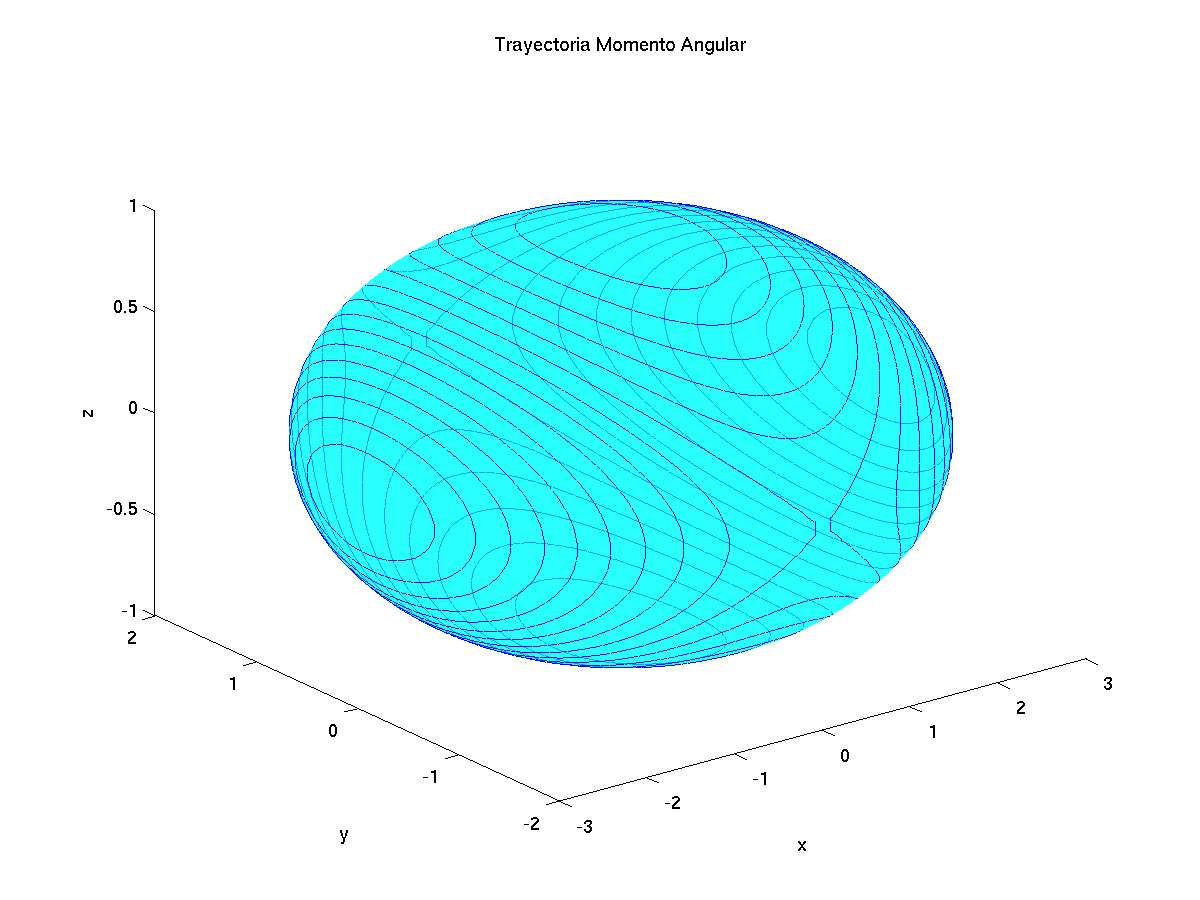
\includegraphics[width=10cm]{Figuras/Intersecciones Elipsoide - EsferaotroDT2.png}
\caption{Intersecciones Elipsoide - Esfera}
\label{fig:cinemat_Intersecciones_Elipsoide_Esfera}
\end{figure}
% ------------------------------------

\subsection{Posibles situaciones}
\label{sec:cinemat_posibles_situaciones_interseccion_elipsoide_esfera}

Del sistema de Ec.(\ref{eq:cinemat_sist_energia_y_momento}) para una cantidad de energ\'ia constante existen distintas situaciones posibles, principalmente definidas por los tres semi-ejes, los cuales justamente se corresponden a los ejes principales de inercia, Fig,(\ref{fig:cinemat_Intersecciones_Elipsoide_Esfera}). Para ello se procede a an\'alizar las posibles soluciones, partiendo del valor m\'inimo hasta el valor m\'aximo que puede adoptar el momento, es decir $c^2<M^2<a^2$.

\subsubsection{Intersecci\'on sobre semi-eje menor}
\label{sec:cinemat_Interseccion_sobre_semi-eje_menor}


% se comentan las dos fotos por separados, xq no funciona el subplot
\begin{comment}
% ------------------------------------
\begin{figure}[H]
\centering
\includegraphics[width=10cm]{figs/Cinematica/Trayectoria Momento - Inercia I_3.png}
\caption{Trayectoria Momento - Inercia $I_3$}
\label{fig:cinemat_Trayectoria_Momento_Inercia I_3}
\end{figure}
% ------------------------------------
% ------------------------------------
\begin{figure}[H]
\centering
\includegraphics[width=10cm]{figs/Cinematica/Trayectoria Momento - Inercia I_1.png}
\caption{Trayectoria Momento - Inercia $I_1$}
\label{fig:cinemat_Trayectoria_Momento_Inercia I_1}
\end{figure}
% ------------------------------------
\end{comment}



En primer lugar cuando el cuerpo se encuentra girando sobre su menor eje principal de inercia $2EI_3$, este se encuentra colineal con su velocidad angular $|\vec{\Omega}|$, y es proporcional al $|\vec{M}|$, esto se debe a que el vector momento se encuentra alineado con la velocidad angular. 

Ahora si el momento tiene una componente que interrumpe esa colinealidad, es decir el $|\vec{M}|$ sufre una m\'inima variaci\'on respecto al eje de inercia, Fig.(\ref{fig:cinemat_Trayectoria_Momento_inercias_estables_I1_I3}a), en este caso la soluci\'on del sistema energ\'ia-momento ser\'an dos circunferencias. Estas curvas son la soluci\'on de la intersecci\'on entre el elipsoide de energ\'ia y la esfera de momento; una circunferencia por cada lado del elipsoide. En este caso, el vector momento $|\vec{M}|$ al desplazarse sobre dicha curva realiza un movimiento en forma de cono. A dicho fen\'omeno se lo conoce como fen\'omeno de \textit{precesi\'on} y se define como el movimiento asociado al cambio de direcci\'on que experimenta el eje instant\'aneo de rotaci\'on. En otras palabras es un \underline{par\'ametro que indica cu\'an desalineado se encuentra el} \underline{vector momento $|\vec{M}|$ de los ejes principales de inercia}.
Si bien en Sec.(\ref{sec:cinemat_asymmetrical_top_precesion}) se realiza el an\'alisis matem\'atico del fen\'omeno de precesi\'on para un cuerpo \texttt{symetrical-top}, dicho fen\'omeno ocurre tambi\'en en los cuerpos \texttt{asymmetrical-top} cuando sufren una variaci\'on del momento $\vec{M}$ cercana al menor eje de inercia\footnote{Del desarrollo se manifiesta que el fen\'omeno precesi\'on ocurre tanto para el menor eje de inercia $I_3$ como para el mayor $I_1$}.

A medida que dicha desalineaci\'on aumenta, el grado de apertura del cono ser\'a mayor, ya que aumenta la circunferencia dada por la intersecci\'on entre el elipsoide y la esfera. En dicho caso, el vector $\vec{M}$ sufrir\'a una modificaci\'on en sus componentes. Si bien se dijo con anterioridad que su m\'odulo es constate $|\vec{M}|=C_1$, siendo $C_1\epsilon CT(0)$, no obstante el vector $\vec{M}=\vec{M}_1+\vec{M}_2+\vec{M}_3$, por lo que sus componentes se modificar\'an. En consecuencia, la proyecci\'on sobre el eje principal de inercia ser\'a menor y por ende el cuerpo sufri\'ra una disminuci\'on en su velocidad angular, mientras que dicha diferencia contribuir\'a en el movimiento de precesi\'on, realizando una curva circular m\'as pronunciada. Estas situaciones se pueden deducir de la Fig.(\ref{fig:cinemat_omega_vectorial_t=pi/(2omega_pr)} y Fig.(\ref{fig:cinemat_momento_vectorial_t=pi/(2omega_pr)}).

%Es decir, el vector momento se confecciona mediante la contribuci\'on de dos vectores, el vector colineal al eje de rotaci\'on $\vec{M}_3 \simeq \vec{\Omega}_3= \vec{\Omega}_{pr}$ y la otra componente del vector es  $\vec{M}_A=\vec{M}_1+\vec{M}_2\simeq\vec{\Omega_A}$ las cuales sumadas vectorialmente resulta en el vector momento $\vec{M}=\vec{M}_{pr}+\vec{M}_A$, Fig.(\ref{fig:cinemat_Esquema vectorial_precesion}). Por lo tanto cuanto m\'as pronunciado sea la apertura del cono, mayor ser\'a la contribuci\'on del vector momento $\vec{M}_A$, sobre el vector $\vec{M}$ y en consecuencia, menor la contribuci\'on de la componente de precesi\'on, $\vec{M}_{pr}\simeq \vec{\Omega}_3$, lo que se traduce en una disminuci\'on de la rotaci\'on respecto al eje de inercia $I_3$.


% ------------------------------------
\begin{figure}[H]
\centering
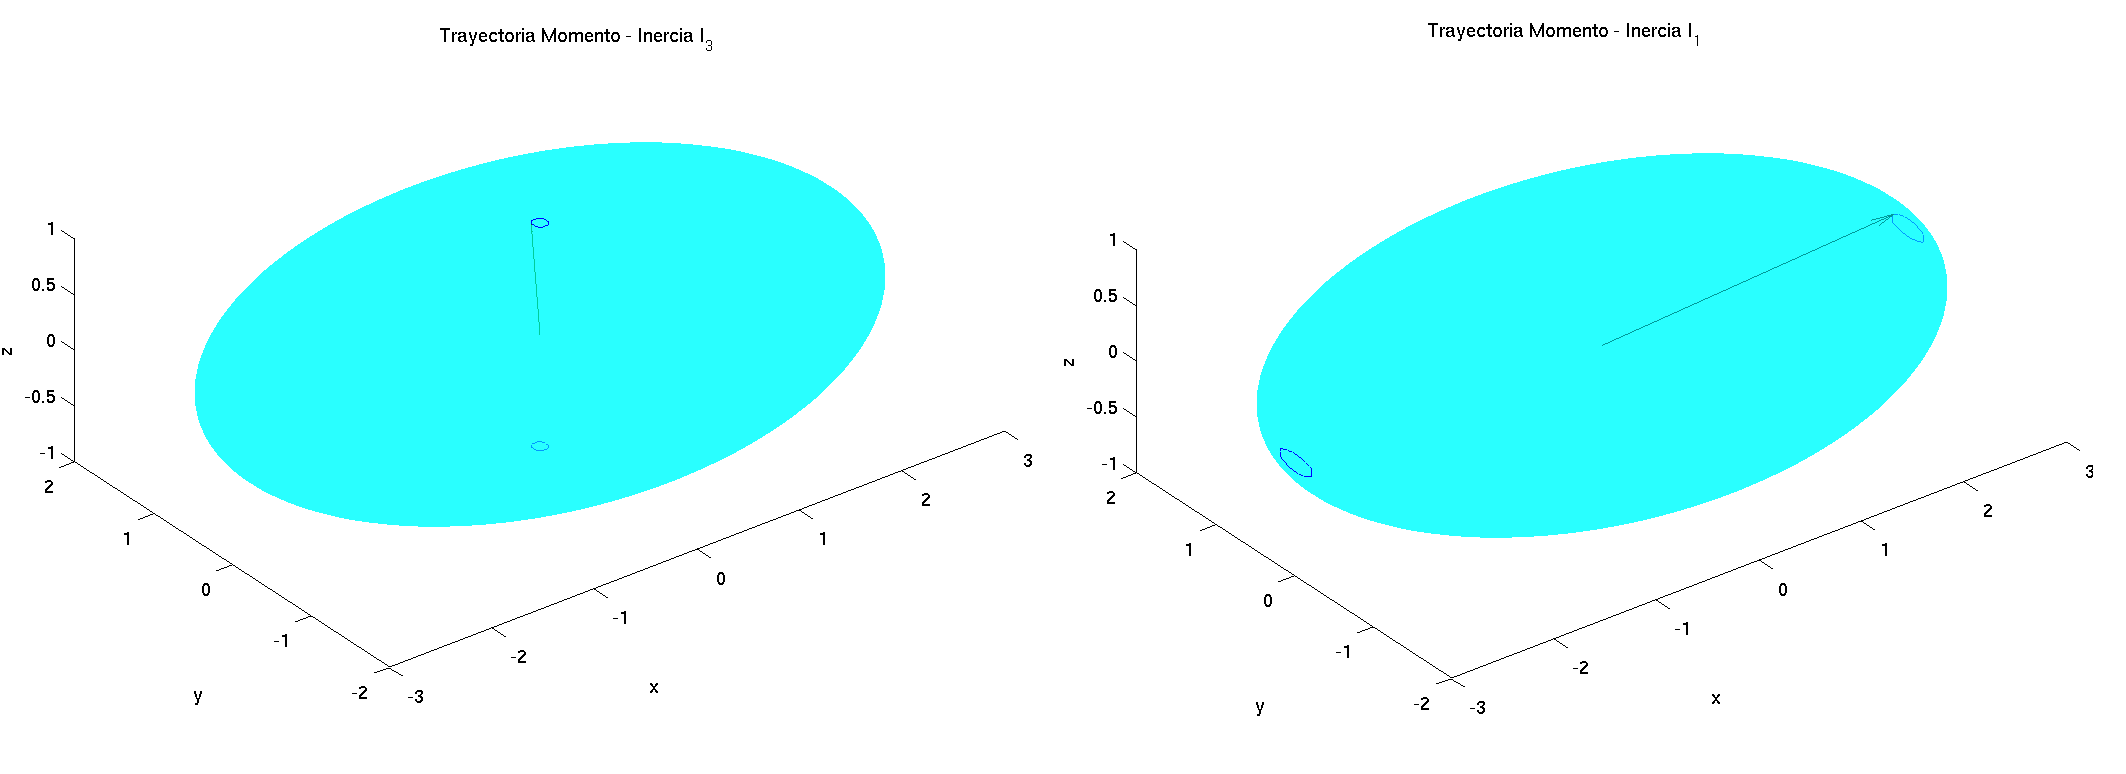
\includegraphics[width=17cm]{Figuras/inercias_estables_I1_I3.png}
\caption{Trayectoria Estable Momento Inercia, $I_1$ y $I_3$}
\label{fig:cinemat_Trayectoria_Momento_inercias_estables_I1_I3}
\end{figure}
% ------------------------------------

La interpretaci\'on gr\'afica del fen\'omeno de \texttt{precesi\'on} se aprecia cuando la circunferencia dada por la intersecci\'on entre el elipsoide y la esfera comienza a crecer y por ende la proyecci\'on del vector momento $\vec{M}$ sobre el eje de inercia  comienza a disminuir. Visto de otra manera, cuanto m\'as alineado se encuentra el vector $|\vec{M}|$ respecto al eje de rotaci\'on, mayor ser\'a su proyecci\'on sobre este, y por ende mayor ser\'a su velocidad de rotaci\'on $|\vec{\Omega}|$. Como la intersecci\'on entre la elipse y la esfera es una curva cerrada se evidencia que el movimiento del vector momento $|\vec{M}|$ es per\'iodico, es decir el vector se desplaza por el camino descripto por la curva intersecci\'on y luego vuelve a su posici\'on original.


Esta situaci\'on en la cual una peque\~na variaci\'on de la curva descripta por el vector momento $|\vec{M}|$ produce una desviaci\'on pr\'oxima a la situaci\'on anterior, ocurre tanto en los semi-ejes mayor ($I_1$) y menor ($I_3$) de la elipse, Fig.(\ref{fig:cinemat_Trayectoria_Momento_inercias_estables_I1_I3}). No obstante se observa que la situaci\'on sobre la regi\'on cercana al eje intermedio ($I_2$), la curva descripta es distinta a una circunferencia cercana al eje de inercia, Fig.(\ref{fig:cinemat_Trayectoria_Momento_Inercia I_2}). En el caso en que el cuerpo se encuentra rotando sobre el eje intermedio de inercia ($I_2$) y experimenta una leve variaci\'on sobre el momento $|\vec{M}|$, este tendr\'a un comportamiento cualitativamente diferente, donde el camino recorrido por el vector momento $|\vec{M}|$ realiza una trayectoria totalmente extra\~na y alejada de los "polos" de dicho semi-eje.

% ------------------------------------
\begin{figure}[H]
\centering
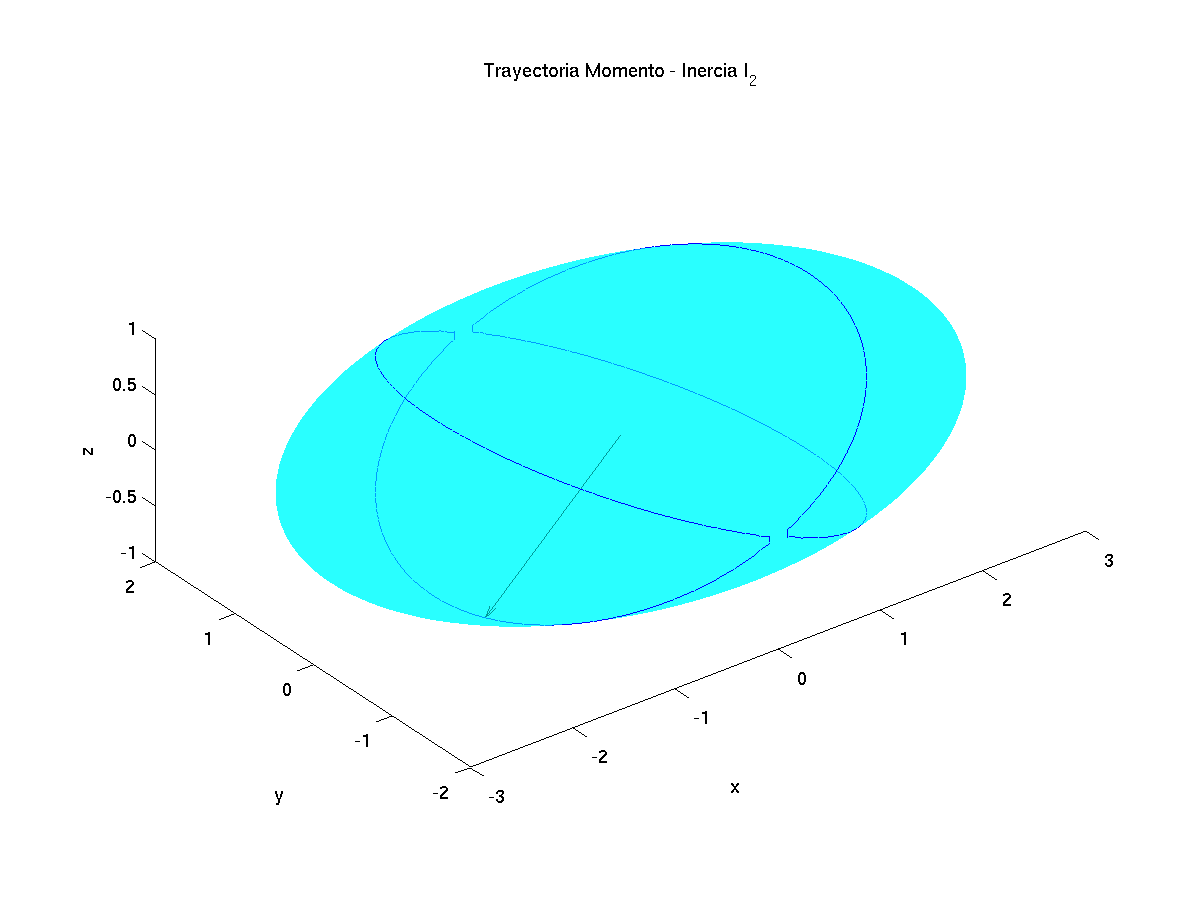
\includegraphics[width=10cm]{Figuras/Trayectoria Momento - Inercia I_2.png}
\caption{Trayectoria Momento - Inercia $I_2$}
\label{fig:cinemat_Trayectoria_Momento_Inercia I_2}
\end{figure}
% ------------------------------------

Esta situaci\'on anterior se debe a que el movimiento de rotaci\'on del cuerpo sobre los semi-ejes mayor ($I_1$) y menor ($I_3$) es estable, mientras que el movimiento de rotaci\'on respecto al eje intermedio ($I_2$) es inestable, generando esa extra\~na y asombrosa perturbaci\'on descripta durante el giro en dicha situaci\'on. Esta fen\'omeno se conoce como paradoja de la raqueta de tennis o teorema del eje intermedio, tambi\'en conocido como efecto 'Dzhanibekov' o efecto Wingnut y gr\'aficamente se manifiesta que dicha trayectoria bizarra se debe a la intersecci\'on entre el elipsoide y la esfera que ocurre cercano al segundo eje principal de inercia, Fig(\ref{fig:cinemat_Trayectoria_Momento_Inercia I_2}).


%------------------------------------------
\section{Metodología}
\label{sec:metodologia}

Para  hacer frente a las cuestiones t\'ecnicas se desarroll\'o un algoritmo que resuelve el modelo de RBD (Rigid Body Dynamics, 'Din\'amica de Cuerpo R\'igido') con 6DOF's (Degrees of Freedom, 'Grados de Libertad') el cual utiliza cuaterniones para la representaci\'on matem\'atica de las orientaci\'on del cuerpo. Esto \'ultimo es una ventaja ya que dicha modelizaci\'on permite capturar desplazamientos en cualquier direcci\'on, cuesti\'on que no es posible si se utilizan los \'angulos de Euler debido a la singularidad conocida como \textit{gimbal-lock}\footnote{El \textit{gimbal-lock}consiste en la pérdida de un grado de libertad en una suspensión cardán de tres rotores, que ocurre cuando los ejes de dos de los tres rotores se colocan en paralelo, bloqueando el sistema en una rotación en un espacio bidimensional degenerado}.

El algoritmo resuelve las ecuaciones de Euler, Ec.(\ref{eq:cinemat_ODEs_vel_angular_sin_torques_ecternos}) y modeliza la trayectoria de un cuerpo bajo las condiciones iniciales de movimiento. Se encuentra implementado en el lenguaje \texttt{python} y para resolver las ODE's se utiliza un integrador temporal con paso de tiempo adaptativo. El mismo se abastece de los par\'ametros f\'isicos del objeto como ser sus par\'ametros geom\'etricos, inercia, centro de masa, etc. El modelo devuelve como resultado los valores num\'ericos de la trayectoria y gr\'aficas que manifiesta la evoluci\'on de los par\'ametros involucrados.



%-------------------------------------------
\section{Resultados}
\label{sec:resultados}

\subsection{Simulaci\'on Num\'erica}

Se realizan las simulaciones num\'ericas sobre las cuales se omiten las traslaciones ya que dichos valores no inciden sobre los efectos de la rotaci\'on. El objeto seleccionado fue un objeto \textit{asymmetrical-top} con las caracter\'isticas que se presentan en la Fig.(\ref{fig:carac_objeto_wingnut}).


\begin{figure}[h]
\begin{subfigure}{.55\textwidth}
  \centering
  % include first image
  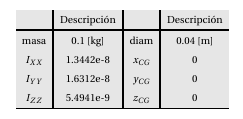
\includegraphics[width=.7\linewidth]{Figuras/detalles_wingnut.png}
  \caption{Caracter\'isticas Tuerca Wingnut}
  \label{fig:carac_tuerca_wingnut}
\end{subfigure}
\begin{subfigure}{.55\textwidth}
  \centering
  % include second image
  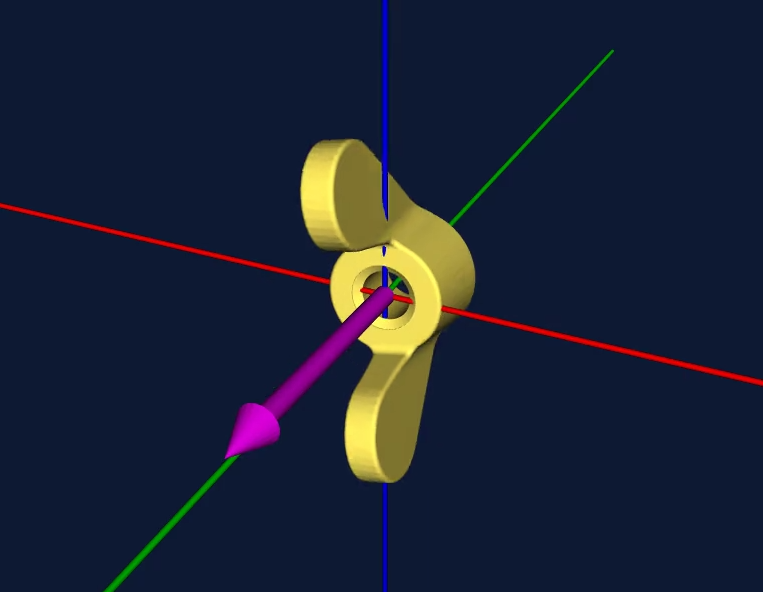
\includegraphics[width=.6\linewidth]{Figuras/wingnut.png}
  \caption{Isometr\'ia Wingnut}
  \label{fig:isometria_wingnut}
\end{subfigure}
\caption{Objeto Asymmetrical-top}
\label{fig:carac_objeto_wingnut}
\end{figure}


Las figuras Fig.(\ref{fig:recorrido_trayectoria_momento_rotado_simil_video_mario}) y Fig(\ref{fig:resultado_wingnut_video_mario}) representan las trayectorias que recorre el vector momento $\vec{M}$ lo cual concuerda con la inestabilidad explicada en Sec.(\ref{sec:cinemat_Interseccion_sobre_semi-eje_menor}). 

\begin{figure}[h]
\begin{subfigure}{.55\textwidth}
  \centering
  % include first image
  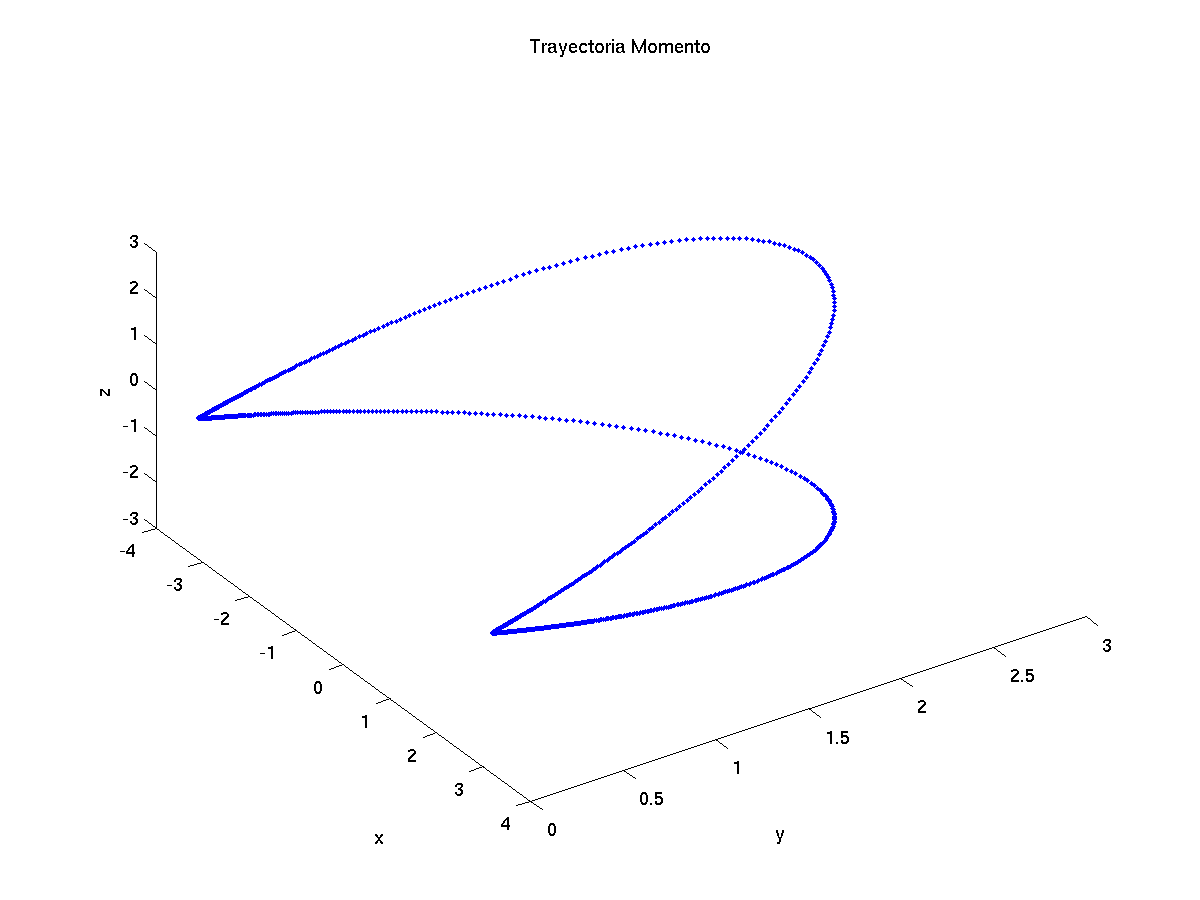
\includegraphics[width=.77\linewidth]{Figuras/Recorrido_Vel_angular_Body_rotada_simil_video.png}
  \caption{Trayectoria Vector Momento, $\vec{M}$}
  \label{fig:recorrido_trayectoria_momento_rotado_simil_video_mario}
\end{subfigure}
\begin{subfigure}{.55\textwidth}
  \centering
  % include second image
  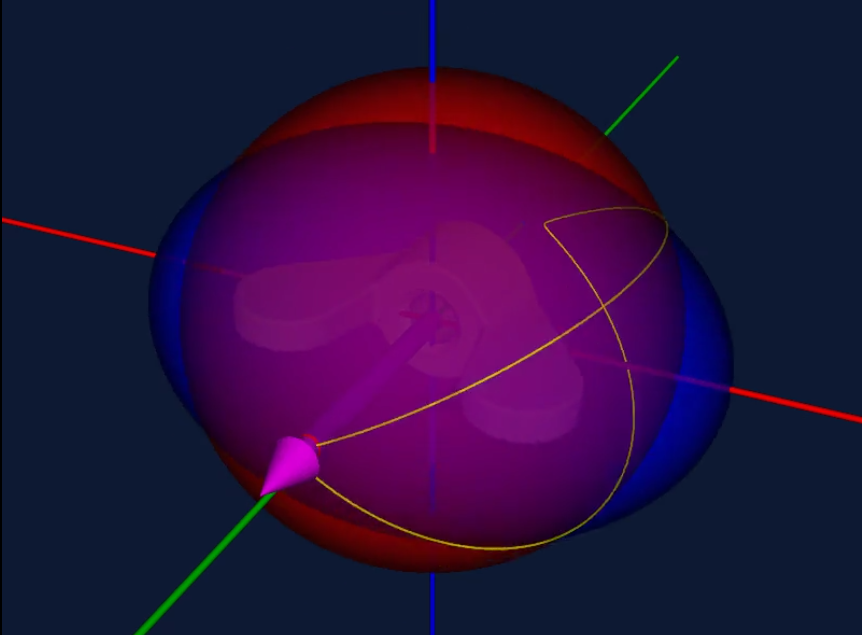
\includegraphics[width=.77\linewidth]{Figuras/fig22.png}
  \caption{Resultado Wingnut}
  \label{fig:resultado_wingnut_video_mario}
\end{subfigure}
\caption{Esquemas resultados sobre situaci\'on real}
\label{fig:recorrido_vector_momento_subfigures_matlab_y_video_mario}
\end{figure}



\subsection{Secuencia de rotaci\'on, Inestabilidad eje intermedio}
\label{sec:secuencia_inestabilidad_eje_intermedio}

En la Fig.(\ref{fig:secuencia_rotacion_inestabilidad_dzhanibekov_effect_wingnut}) se presenta la secuencia de rotaciones que manifiesta la inestabilidad que experimenta un cuerpo \textit{asymmetrical-top} cuando rota respecto a su eje intermedio. Para una mejor comprensi\'on se representa la rotaci\'on sobre la cual a medida que se va desarrollando la misma se comienza a colocar los disitintos par\'ametros que se encuentran  presentes, como ser: el elipsoide de energ\'ia, la esfera de momento, el vector momento y la trayectoria que este describe. El vector de color magenta representa el vector momento, $\vec{M}$, el cual en todo instante sigue la trayectoria dada por la intersecci\'on entre el elipsoide de energ\'ia y la esfera de momento. Para una mayor comprensi\'on visual se representa a la elipsoide de energ\'ia de color azul, mientras que la esfera de momento, es de color rojo. Se aprecia que la intersecci\'on entre las dos curvas (elipsoide-esfera) es la trayectoria descripta en la Fig.(\ref{fig:recorrido_vector_momento_subfigures_matlab_y_video_mario}).


% ------------------------------------
\begin{figure}[H]
\centering
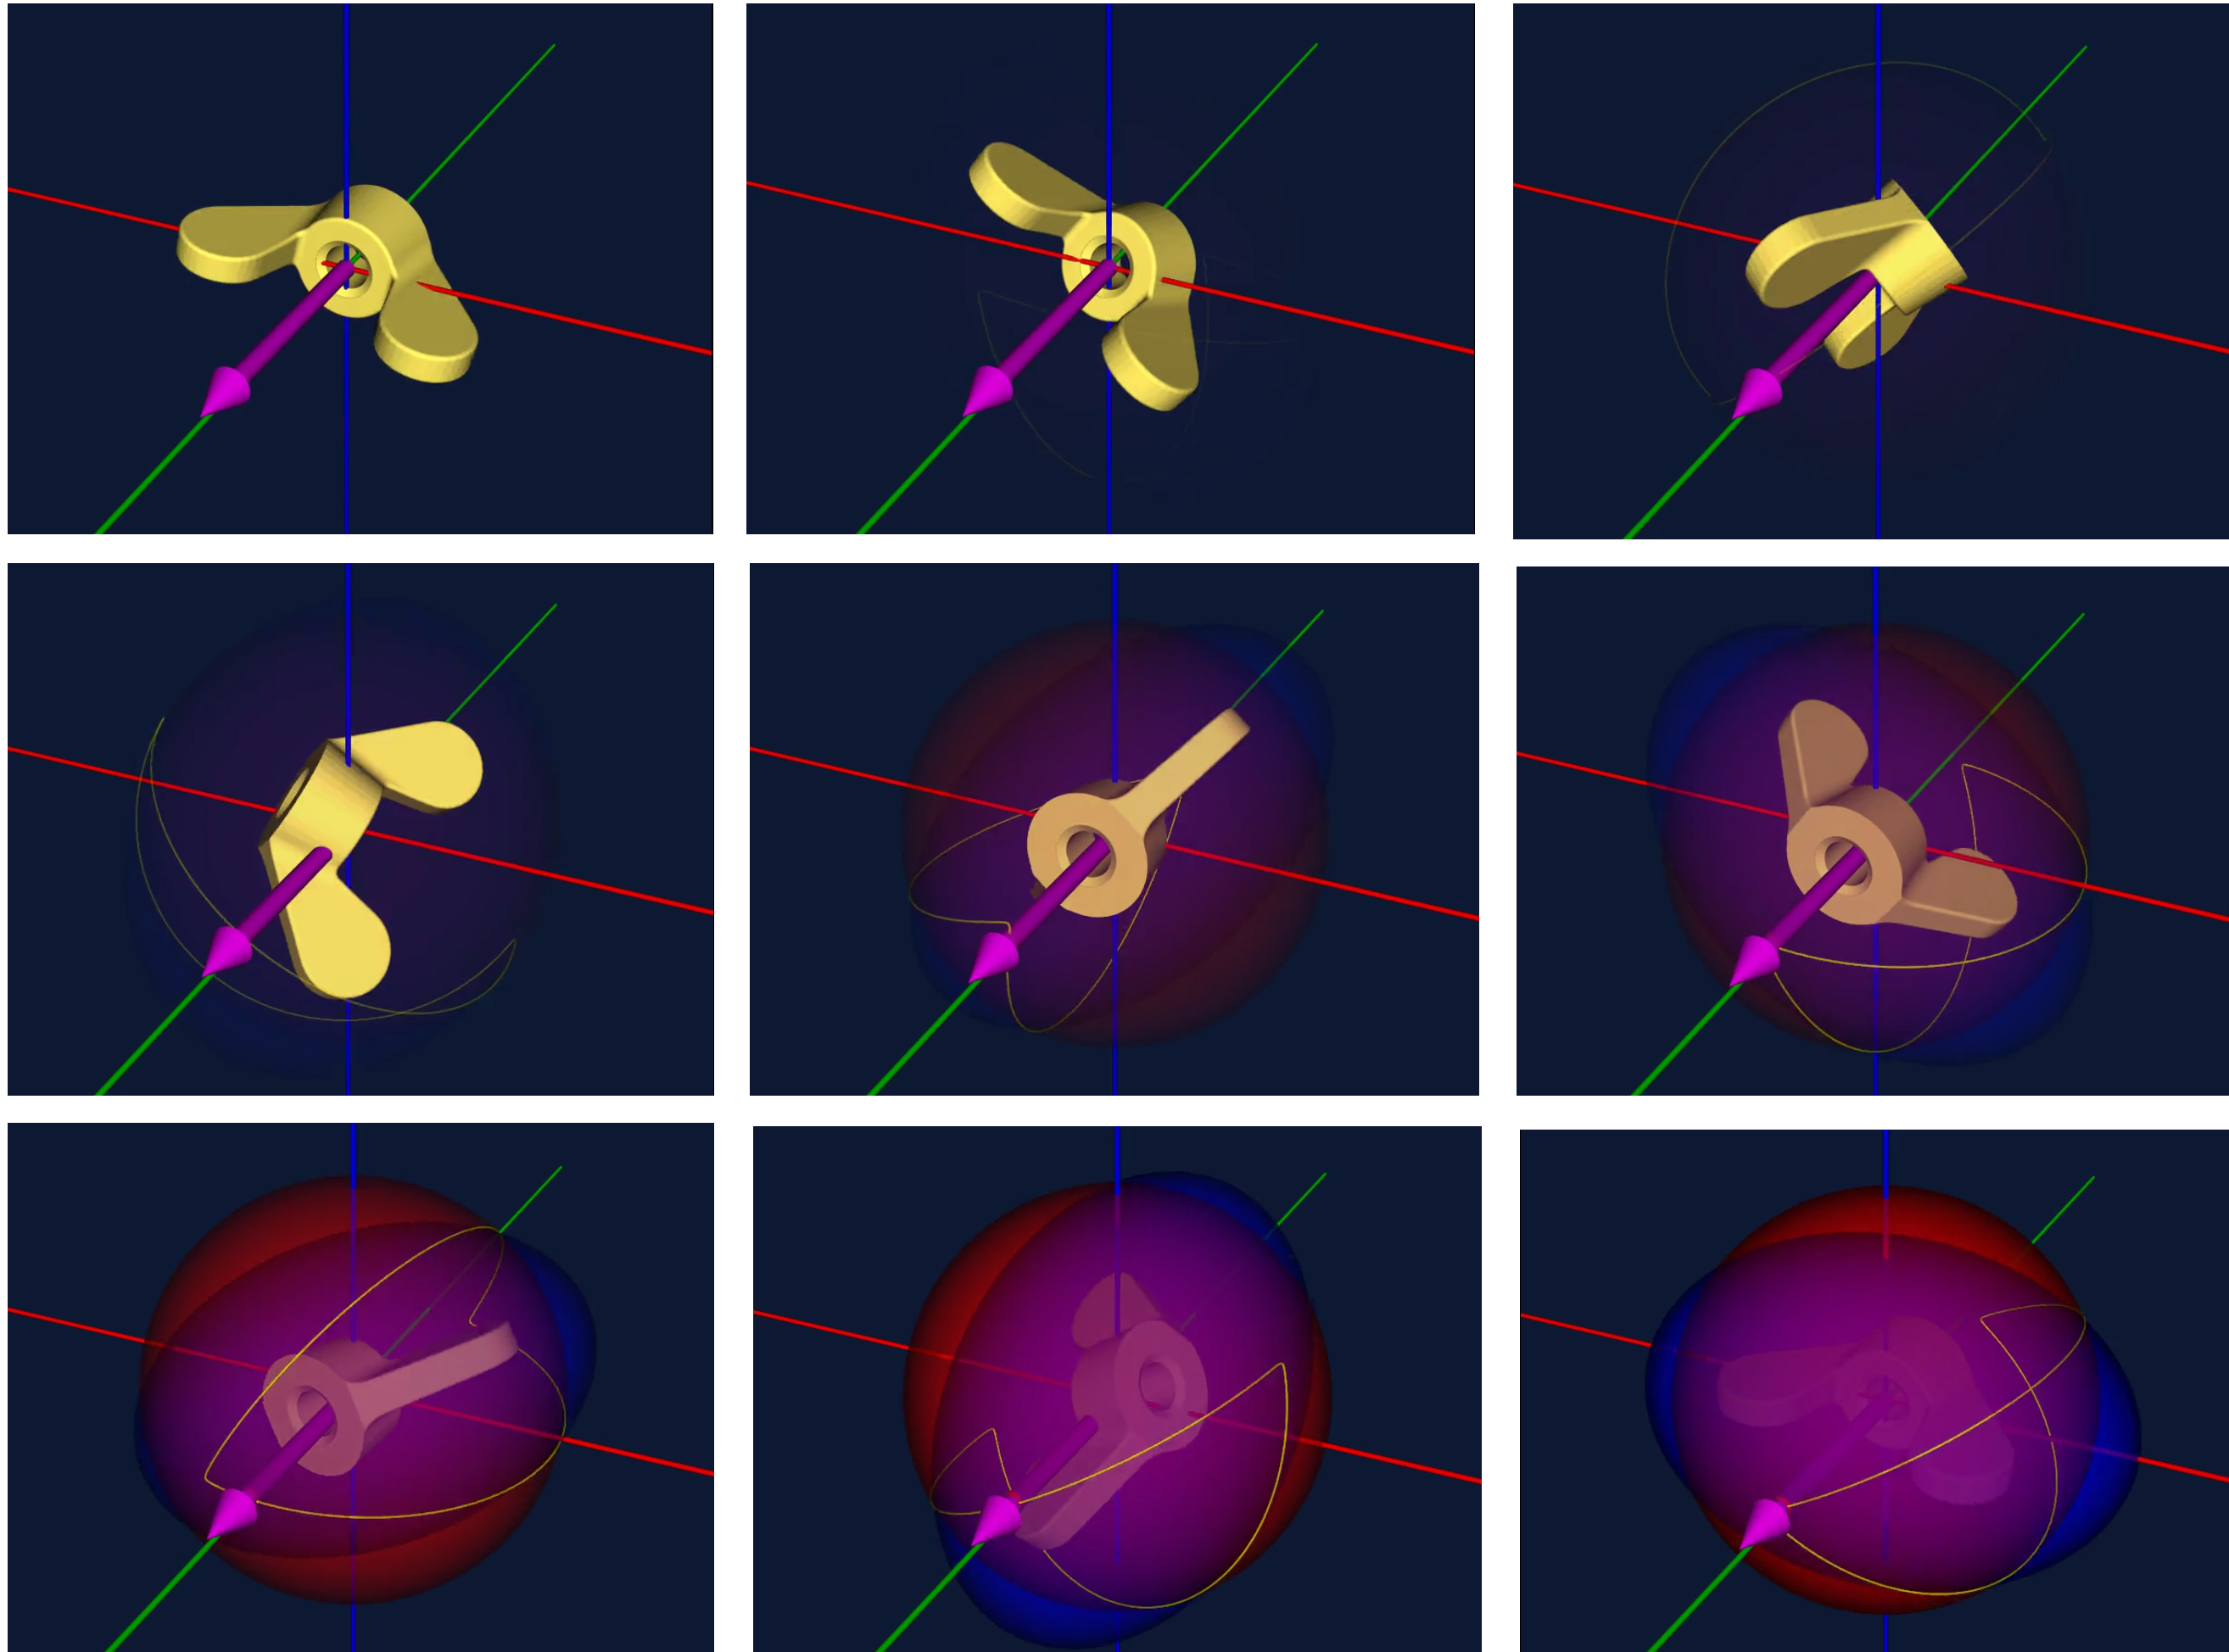
\includegraphics[width=15cm]{Figuras/secuencia_rotacion_inestabilidad.png}
\caption{Secuencia de rotaci\'on -  Inestabilidad del eje intermedio, Dzhanibekov effect}
\label{fig:secuencia_rotacion_inestabilidad_dzhanibekov_effect_wingnut}
\end{figure}
% ------------------------------------



\begin{comment}
% - - - - - - - - - - - - - - - - - - -
\section{otros- Comentarios para agregar}

\hl{notas para activar visualizacion}
Para que funcione la visualizacion para cualquier stl, se debe activar el pythonpath que llama a las librerias de mario y comentar el pythonpath que llama a las librerias de estimacion(python3 con casadi, etc). Esto es en el ./bashrc se debe tener:
\begin{verbatim}
export PYTHONPATH=$HOME/Documents/CIMEC/Tesis/2019/popurri/
testing_viz_vtk/viz/python/

#export PYTHONPATH=/home/zeeburg/Softwares/:
\end{verbatim}

y ejecutar el prog \texttt{python viz2 stl.py} en el path \texttt{/home/zeeburg/Documents/CIMEC/
Tesis/2019/popurri/testing viz vtk/viz}
\end{comment}




%-------------------------------------------
\section{Conclusiones}

Se desarrolla un algoritmo que modeliza la din\'amica de un cuerpo r\'igido, RBD y sobre el mismo se analizan las rotaciones de un cuerpo respecto a sus tres ejes de inercia. Se demuestra que para el caso de un cuerpo \textit{asymmetrical-top} las rotaciones respecto al $1^{er}$ y $3^{er}$ eje de inercia son estables. Sin embargo, las rotaciones respecto al eje de inercia intermedio presentan una pertubaci\'on debido a una inestabilidad sobre dicha rotaci\'on. A este fen\'omeno se lo conoce como inestabilidad del eje intermedio, paradoja de la raqueta de tennis o efecto 'Dzhanibekov'. Se obtiene la soluci\'on del sistema de ODE's mediante un enfoque geom\'etrico obteni\'endose de este modo un camino alternativo al an\'alizar estabilidad de ecuaciones diferenciales.


\newpage
\bibliographystyle{apalike}
\bibliography{Bibliografia.bib}

% ------------------------------------
\end{document}




